%1. 规范硕士导言
\documentclass[master,ttf]{nudtpaper}
%2. 规范博士导言
% \documentclass[doctor,twoside,ttf]{nudtpaper}

% \documentclass[doctor,twoside,fz]{nudtpaper}
%4. 如果想生成盲评,传递anon即可,仍需修改个人成果部分
% \documentclass[master,otf,anon]{nudtpaper}
%
% \documentclass[master,otf]{nudtpaper}
\usepackage{mynudt}

\classification{TP957}
\serialno{18070059}
\confidentiality{公开}
\UDC{}
\title{载人探月飞船返回再入研究}
\displaytitle{载人探月飞船返回再入研究}
\author{周亮}
\zhdate{\zhtoday}
\entitle{How to Use the \LaTeX{} Document Class for NUDT Dissertations}
\enauthor{ZHOU Liang}
\endate{\entoday}
\subject{航空宇航科学与技术}
\ensubject{Aeronautical and Astronautical Sicence and Technology}
\researchfield{飞行动力学与控制}
\supervisor{张洪波\quad{}教授}
\cosupervisor{} % 没有就空着
\ensupervisor{Prof. ZHANG Hongbo}
\encosupervisor{} % 没有就空着
\papertype{工学}
\enpapertype{Engineering}
% 加入makenomenclature命令可用nomencl制作符号列表。

\graphicspath{{figures/}}
\begin{document}

% 制作封面,生成目录,插入摘要,插入符号列表 \\
% 默认符号列表使用denotation.tex,如果要使用nomencl \\
% 需要注释掉denotation,并取消下面两个命令的注释。 \\
% cleardoublepage% \\
% printnomenclature% \\
\maketitle
\frontmatter
% \tableofcontents
% \listoftables
% \listoffigures

% 如果不是送审论文,则将true改为false即可
%\newif\ifreview\reviewtrue
\newif\ifreview\reviewfalse
\midmatter
% \begin{cabstract}
国防科学技术大学是一所直属中央军委的综合性大学。1984年,学校经国务院、中央军委和教育部批准首批成立研究生院,%
肩负着为全军培养高级科学和工程技术人才与指挥人才,培训高级领导干部,从事先进武器装备和国防关键技术研究的重要任务。%
国防科技大学是全国重点大学,也是全国首批进入国家“211工程” 建设并获中央专项经费支持的全国重点院校之一。%
学校前身是1953年创建于哈尔滨的中国人民解放军军事工程学院,简称“哈军工”。
\end{cabstract}
\ckeywords{国防科学技术大学; 211; 哈军工}

\begin{eabstract}
National University of Defense Technology is a comprehensive national key university based in Changsha, %
Hunan Province, China. It is under the dual supervision of the Ministry of National Defense %
and the Ministry of Education, designated for Project 211 and Project 985, %
the two national plans for facilitating the development of Chinese higher education. %

NUDT was originally founded in 1953 as the Military Academy of Engineering in Harbin of Heilongjiang Province. %
In 1970 the Academy of Engineering moved southwards to Changsha and was renamed Changsha Institute of Technology.%
 The Institute changed its name to National University of Defense Technology in 1978.

\end{eabstract}
\ekeywords{NUDT; MND; ME}


% \chapter*{符号使用说明}
% 可以根据需要在chapter后加星星/去掉星星

\begin{denotation}

\item[HPC] 高性能计算 (High Performance Computing)
\item[cluster] 集群
\item[Itanium] 安腾
\item[SMP] 对称多处理
\item[API] 应用程序编程接口
\item[PI]	聚酰亚胺
\item[MPI]	聚酰亚胺模型化合物,N-苯基邻苯酰亚胺
\item[PBI]	聚苯并咪唑
\item[MPBI]	聚苯并咪唑模型化合物,N-苯基苯并咪唑
\item[PY]	聚吡咙
\item[PMDA-BDA]	均苯四酸二酐与联苯四胺合成的聚吡咙薄膜
\item[$\Delta G$]  	活化自由能~(Activation Free Energy)
\item [$\chi$] 传输系数~(Transmission Coefficient)
\item[$E$] 能量
\item[$m$] 质量
\item[$c$] 光速
\item[$P$] 概率
\item[$T$] 时间
\item[$v$] 速度

\end{denotation}


%书写正文,可以根据需要增添章节; 正文还包括致谢,参考文献与成果
\mainmatter
% \chapter{第一章题目}

本章的主要内容与学校提供的Word模板中内容一致,图片与表格均采用原始设定大小,%
主要是为了说明格式的统一。%
但是,\LaTeX{}的一些禁则,专业排版的能力,对公式及文献的处理都是得天独厚的,%
我们不必刻意去追求与Word的完美匹配。而且你将会发现,用\LaTeX{}书写论文的美! %

\section{(1.1 题目)}
正文内容

\subsection{(1.1.1 题目)}
正文内容

正文内容

\begin{figure}[htp]
\centering
\includegraphics{picmain}
\caption{图 1.1 名称}
\end{figure}

\subsubsection{(1.1.1.1 题目)}
正文内容

正文内容

正文内容

\subsubsection{(1.1.1.2 题目)}
正文内容

正文内容

正文内容

\subsection{(1.1.2 题目)}
正文内容

正文内容

\begin{figure}[htp]
\centering
\includegraphics{picmain}
\caption{图 1.2 名称}
\end{figure}

\section{(1.2 题目)}
正文内容

正文内容

\begin{table}[htp]
\centering
\caption{表 1.2 名称}
\begin{tabular}{|c|c|c|c|c|}
\hline
\makebox[2.07cm][0pt]{} & \makebox[2.07cm][0pt]{} & \makebox[2.07cm][0pt]{} & \makebox[2.07cm][0pt]{} & \makebox[2.07cm][0pt]{} \\
\hline
 & & & & \\
\hline
 & & & & \\
\hline
\end{tabular}
\end{table}

正文内容

正文内容

正文内容

正文内容

\section{(1.3 题目)}
正文内容

正文内容

正文内容

正文内容

正文内容

正文内容

\subsection{(1.3.1 题目)}
正文内容

\begin{figure}[htp]
\centering
\includegraphics{picmain}
\caption{图 1.3 名称}
\end{figure}

\subsection{(1.3.2 题目)}
正文内容

正文内容

\begin{table}[htp]
\centering
\caption{表 1.2 名称}
\begin{tabular}{|c|c|c|c|c|}
\hline
\makebox[2.07cm][0pt]{} & \makebox[2.07cm][0pt]{} & \makebox[2.07cm][0pt]{} & \makebox[2.07cm][0pt]{} & \makebox[2.07cm][0pt]{} \\
\hline
 & & & & \\
\hline
 & & & & \\
\hline
\end{tabular}
\end{table}


% \chapter{论文正文}
\label{chap:main}
本章将进入论文排版的正文, 按元素分主要包括:
{\kai 字体段落,图片表格,公式定理,参考文献}这几部分。
这个样例文件将包括模板中使用到的所有格式、模板中自定义命令到或者特有的东西,
都将被一一介绍,希望大家在排版自己的学位论文前能细致的看一遍,记住样例的格式和
方法,方便上手。

\section{字体段落}
\label{sec:font}

陈赓(1903年2月27日-1961年3月16日),原名陈庶康,中国湖南湘乡人,军事家。出生将门,其祖父为湘军将领陈翼怀。

Adobe中文字体有四种:

{\kai 楷体\verb|\kai|:陈赓,中国湖南湘乡人,军事家。出生将门,其祖父为湘军将领陈翼怀。%
1952年筹办并任人民解放军军事工程学院第一任院长兼政委,培养国防科技人才。1955年被授予大将军衔。}

{\fs 仿宋\verb|\fs|:陈赓,中国湖南湘乡人,军事家。出生将门,其祖父为湘军将领陈翼怀。%
1952年筹办并任人民解放军军事工程学院第一任院长兼政委,培养国防科技人才。1955年被授予大将军衔。}

{\hei 黑体\verb|\hei|:陈赓,中国湖南湘乡人,军事家。出生将门,其祖父为湘军将领陈翼怀。%
1952年筹办并任人民解放军军事工程学院第一任院长兼政委,培养国防科技人才。1955年被授予大将军衔。}

宋体就是正文字体了。下面测试字体大小,\LaTeX{}默认的列表环境会在
条目之间插入过多的行距,在下面这种情况可能正好,若用户需要
{\kai 正文行距}的列表环境,可以使用compactitem环境,记住这点很重要,不要再
用那种自己修改\verb|itemsep|的傻傻的办法了。
\begin{itemize}
  \item[初号] {\song\chuhao 陈赓大将}
  \item[小初] {\song\xiaochu 陈赓大将}
  \item[一号] {\song\yihao 陈赓大将}
  \item[小一] {\song\xiaoyi 陈赓大将}
  \item[二号] {\song\erhao 陈赓大将}
  \item[小二] {\song\xiaoer 陈赓大将}
  \item[三号] {\song\sanhao 陈赓大将}
  \item[小三] {\song\xiaosan 陈赓大将}
  \item[四号] {\song\sihao 陈赓大将}
  \item[小四] {\song\xiaosi 陈赓大将}
  \item[五号] {\song\wuhao 陈赓大将}
  \item[小五] {\song\xiaowu 陈赓大将}
\end{itemize}

\section{表格明细}
\label{sec:figure}
表格是论文的重要组成部分,我们从简单的表格讲起,到复杂的表格为止。

模板中关于表格的宏包有三个: \textsf{booktabs}、\textsf{array} 和
\textsf{longtabular}。三线表建议使用\textsf{booktabs}中提供的,
包含toprule、midrule 和 bottomrule三条命令,简单干脆!
它们与\textsf{longtable} 能很好的配合使用。下面来看一个表格实例:
\begin{table}[htb]
  \centering
  \begin{minipage}[t]{0.8\linewidth} % 如果想在表格中使用脚注,minipage是个不错的办法
    \caption[模板文件]{模板文件。如果表格的标题很长,那么在表格索引中就会很不美
      观,所以要像 chapter 那样在前面用中括号写一个简短的标题。这个标题会出现在索
      引中。}
    \label{tab:template-files}
    \begin{tabular*}{\linewidth}{lp{10cm}}
      \toprule[1.5pt]
      {\hei 文件名} & {\hei 描述} \\
      \midrule[1pt]
      nudtpaper.ins & \LaTeX{} 安装文件,docstrip\footnote{表格中的脚注} \\
      nudtpaper.dtx & 所有的一切都在这里面\footnote{再来一个}。\\
      nudtpaper.cls & 模板类文件。\\
      nudtpaper.cfg & 模板配置文。cls 和 cfg 由前两个文件生成。\\
      bstutf8.bst   & 参考文献 Bibtex 样式文件。\\
      mynudt.sty    & 常用的包和命令写在这里,减轻主文件的负担。\\
      \bottomrule[1.5pt]
    \end{tabular*}
  \end{minipage}
\end{table}

表 \ref{tab:template-files} 列举了本模板主要文件及其功能,基本上来说论文
中最可能用到的就是这种表格形式了。
请大家注意三线表中各条线对应的命令。这个例子还展示了如何在表格中正确使用脚注。
如果你不需要在表格中插入脚注,可以将minipage环境去掉。
由于\LaTeX{}本身不支持在表格中使用\verb|\footnote|,所以我们不得不将表格放在
小页中,而且最好将表格的宽度设置为小页的宽度,这样脚注看起来才更美观。

另外六院的同学在使用模板时需要使用一种固定宽度(往往是页宽,下面的例子由
rongdonghu提供)的表格,内容需要居中且可以自动调整。
解决办法是自定义了一种\verb|tabularx|中的\textbf{Z}环境,在论文模板中,
该命令已添加到\verb|mynudt.sty|中。下面是这种情况的实例:

\begin{table}[htbp]
  \centering
  \begin{minipage}[t]{0.9\linewidth}
    \caption{Reed Solomon码的典型应用}
    \label{tab:RSuse}
    \begin{tabularx}{\linewidth}{cZ}
      \toprule[1.5pt]
      {\hei 应用领域} & {\hei 编码方案}                                          \\
      \midrule[1pt]
      磁盘驱动器      & RS(32,28,5)码 \footnote{码长为32、维数为28、最小距离为5} \\
      CD              & 交叉交织RS码(CIRC)                                       \\
      DVD             & RS(208,192,17)码、RS(182,172,11)码                       \\
      光纤通信        & RS(255,229,17)码                                         \\
      \bottomrule[1.5pt]
    \end{tabularx}
  \end{minipage}
\end{table}

我们经常会在表格下方标注数据来源,或者对表格里面的条目进行解释。前面的脚注是一种
不错的方法,如果你不喜欢minipage方法的脚注。
那么完全可以在表格后面自己写注释,比如表~\ref{tab:tabexamp1}。
\begin{table}[htbp]
  \centering
  \caption{复杂表格示例 1}
  \label{tab:tabexamp1}
  \begin{minipage}[t]{0.8\textwidth}
    \begin{tabularx}{\linewidth}{|l|X|X|X|X|}
      \hline
      \multirow{2}*{\backslashbox{x}{y}} & \multicolumn{2}{c|}{First Half} & \multicolumn{2}{c|}{Second Half}                     \\
      \cline{2-5}
                                         & 1st Qtr                         & 2nd Qtr                          & 3rd Qtr & 4th Qtr \\
      \hline
      \multirow{2}*{East$^{*}$}          & 20.4                            & 27.4                             & 90      & 20.4    \\
                                         & 30.6                            & 38.6                             & 34.6    & 31.6    \\
      West$^{**}$                        & 30.6                            & 38.6                             & 34.6    & 31.6    \\
      \hline
    \end{tabularx}\\[2pt]
    \footnotesize
    *:东部\\
    **:西部
  \end{minipage}
\end{table}

此外,表~\ref{tab:tabexamp1} 同时还演示了另外三个功能:1)通过 \textsf{tabularx} 的
\texttt{|X|} 扩展实现表格内容自动调整;2)通过命令 \verb|\backslashbox| 在表头部分
插入反斜线(WORD中很简单,但\LaTeX{}做表格需要一定的(极大的)想象力);3)就是
使用\verb|multirow|和\verb|multicolumn|命令。

不可否认 \LaTeX{} 的表格功能没有想象中的那么强大,不过只要你足够认真,足够细致,那么
同样可以排出来非常复杂非常漂亮的表格。可是科技论文中那么复杂表格有什么用呢?
上面那个表格就够用啦。

浮动体的并排放置一般有两种情况:1)二者没有关系,为两个独立的浮动体;2)二者隶属
于同一个浮动体。对表格来说并排表格既可以像表~\ref{tab:parallel1}、表~\ref{tab:parallel2}
使用小页环境,也可以如表~\ref{tab:subtable}使用子表格来做。
图与表同出一源,后面我们将讲解子图(subfloat)的例子。
\begin{table}[htb]
  \centering
  \noindent\begin{minipage}{0.45\textwidth}
    \centering
    \caption{第一个并排子表格}
    \label{tab:parallel1}
    \begin{tabular}{p{2cm}p{2cm}}
      \toprule[1.5pt]
      111 & 222 \\\midrule[1pt]
      222 & 333 \\\bottomrule[1.5pt]
    \end{tabular}
  \end{minipage}
  \begin{minipage}{0.45\textwidth}
    \centering
    \caption{第二个并排子表格}
    \label{tab:parallel2}
    \begin{tabular}{p{2cm}p{2cm}}
      \toprule[1.5pt]
      111 & 222 \\\midrule[1pt]
      222 & 333 \\\bottomrule[1.5pt]
    \end{tabular}
  \end{minipage}
\end{table}
\begin{table}[htbp]
  \centering
  \caption{并排子表格}
  \label{tab:subtable}
  \subfloat[第一个子表格]{
    \begin{tabular}{p{2cm}p{2cm}}
      \toprule[1.5pt]
      111 & 222 \\\midrule[1pt]
      222 & 333 \\\bottomrule[1.5pt]
    \end{tabular}}\hskip2cm
  \subfloat[第二个子表格]{
    \begin{tabular}{p{2cm}p{2cm}}
      \toprule[1.5pt]
      111 & 222 \\\midrule[1pt]
      222 & 333 \\\bottomrule[1.5pt]
    \end{tabular}}
\end{table}

如果您要排版的表格长度超过一页,那么推荐使用\textsf{longtable}命令。
这里随便敲入一些无关的文字,使得正文看上去不是那么的少。
表~\ref{tab:performance} 就是 \textsf{longtable} 的简单示例。
\begin{longtable}[c]{c*{6}{r}}
  \caption{实验数据}\label{tab:performance}                                                               \\
  \toprule[1.5pt]
  测试程序 & \multicolumn{1}{c}{正常运行} & \multicolumn{1}{c}{同步}
           & \multicolumn{1}{c}{检查点}   & \multicolumn{1}{c}{卷回恢复}
           & \multicolumn{1}{c}{进程迁移} & \multicolumn{1}{c}{检查点}                                    \\
           & \multicolumn{1}{c}{时间 (s)} & \multicolumn{1}{c}{时间 (s)}
           & \multicolumn{1}{c}{时间 (s)} & \multicolumn{1}{c}{时间 (s)}
           & \multicolumn{1}{c}{时间 (s)} & 文件(KB)                                                    \\
  \midrule[1pt]%
  \endfirsthead%

  \multicolumn{7}{c}{续表~\thetable\hskip1em 实验数据}                                                    \\

  \toprule[1.5pt]
  测试程序 & \multicolumn{1}{c}{正常运行} & \multicolumn{1}{c}{同步}
           & \multicolumn{1}{c}{检查点}   & \multicolumn{1}{c}{卷回恢复}
           & \multicolumn{1}{c}{进程迁移} & \multicolumn{1}{c}{检查点}                                    \\
           & \multicolumn{1}{c}{时间 (s)} & \multicolumn{1}{c}{时间 (s)}
           & \multicolumn{1}{c}{时间 (s)} & \multicolumn{1}{c}{时间 (s)}
           & \multicolumn{1}{c}{时间 (s)} & 文件(KB)                                                    \\
  \midrule[1pt]%
  \endhead%
  \hline%

  \multicolumn{7}{r}{续下页}%

  \endfoot%
  \endlastfoot%
  CG.A.2   & 23.05                        & 0.002                        & 0.116 & 0.035 & 0.589 & 32491  \\
  CG.A.4   & 15.06                        & 0.003                        & 0.067 & 0.021 & 0.351 & 18211  \\
  CG.A.8   & 13.38                        & 0.004                        & 0.072 & 0.023 & 0.210 & 9890   \\
  CG.B.2   & 867.45                       & 0.002                        & 0.864 & 0.232 & 3.256 & 228562 \\
  CG.B.4   & 501.61                       & 0.003                        & 0.438 & 0.136 & 2.075 & 123862 \\
  CG.B.8   & 384.65                       & 0.004                        & 0.457 & 0.108 & 1.235 & 63777  \\
  MG.A.2   & 112.27                       & 0.002                        & 0.846 & 0.237 & 3.930 & 236473 \\
  MG.A.4   & 59.84                        & 0.003                        & 0.442 & 0.128 & 2.070 & 123875 \\
  MG.A.8   & 31.38                        & 0.003                        & 0.476 & 0.114 & 1.041 & 60627  \\
  MG.B.2   & 526.28                       & 0.002                        & 0.821 & 0.238 & 4.176 & 236635 \\
  MG.B.4   & 280.11                       & 0.003                        & 0.432 & 0.130 & 1.706 & 123793 \\
  MG.B.8   & 148.29                       & 0.003                        & 0.442 & 0.116 & 0.893 & 60600  \\
  LU.A.2   & 2116.54                      & 0.002                        & 0.110 & 0.030 & 0.532 & 28754  \\
  LU.A.4   & 1102.50                      & 0.002                        & 0.069 & 0.017 & 0.255 & 14915  \\
  LU.A.8   & 574.47                       & 0.003                        & 0.067 & 0.016 & 0.192 & 8655   \\
  LU.B.2   & 9712.87                      & 0.002                        & 0.357 & 0.104 & 1.734 & 101975 \\
  LU.B.4   & 4757.80                      & 0.003                        & 0.190 & 0.056 & 0.808 & 53522  \\
  LU.B.8   & 2444.05                      & 0.004                        & 0.222 & 0.057 & 0.548 & 30134  \\
  EP.A.2   & 123.81                       & 0.002                        & 0.010 & 0.003 & 0.074 & 1834   \\
  EP.A.4   & 61.92                        & 0.003                        & 0.011 & 0.004 & 0.073 & 1743   \\
  EP.A.8   & 31.06                        & 0.004                        & 0.017 & 0.005 & 0.073 & 1661   \\
  EP.B.2   & 495.49                       & 0.001                        & 0.009 & 0.003 & 0.196 & 2011   \\
  EP.B.4   & 247.69                       & 0.002                        & 0.012 & 0.004 & 0.122 & 1663   \\
  EP.B.8   & 126.74                       & 0.003                        & 0.017 & 0.005 & 0.083 & 1656   \\
  \bottomrule[1.5pt]
\end{longtable}

另外,有的同学不想让某个表格或者图片出现在索引里面,那么请使用命令 \verb|\caption*{}|,
这个命令不会给表格编号,也就是出来的只有标题文字而没有“表~XX”,“图~XX”,否则
索引里面序号{\kai 不连续}就显得不伦不类,这也是 \LaTeX{} 里星号命令默认的规则。

\section{绘图插图}

本模板不再预先装载任何绘图包(如 \textsf{pstricks,pgf} 等),完全由你自己来决定。
个人觉得 \textsf{pgf} 不错,不依赖于 Postscript。此外还有很多针对 \LaTeX{} 的
GUI 作图工具,如 XFig(jFig), WinFig, Tpx, Ipe, Dia, Inkscape, LaTeXPiX,
jPicEdt 等等。本人强烈推荐\textsf{Ipe}。

一般图形都是处在浮动环境中。之所以称为浮动是指最终排版效果图形的位置不一定与源文
件中的位置对应,这也是刚使用 \LaTeX{} 同学可能遇到的问题。
如果要强制固定浮动图形的位置,请使用 \textsf{float} 宏包,
它提供了 \texttt{[H]}(意思是图片就给我放在这里\textcolor{red}{H}ere)参数,
但是除非特别需要,不建议使用\texttt{[H]},而是推荐使用\texttt{[htbp]},
给\LaTeX{}更多选择。比如图~\ref{fig:ipe}。
\begin{figure}[htbp] % use float package if you want it here
  \centering
  \includegraphics[width=3in]{hello}
  \caption{利用IPE制图}
  \label{fig:ipe}
\end{figure}

若子图共用一个计数器,
那么请看图~\ref{fig:big1},它包含两个小图,分别是图~\ref{fig:subfig1}
和图~\ref{fig:subfig2}。这里推荐使用\verb|\subfloat|,{\bf 不要再用}
\verb|\subfigure|和\verb|\subtable|。
\begin{figure}[htb]
  \centering%
  \subfloat[第一个小图形]{%
    \label{fig:subfig1}
    
\includegraphics[height=2cm]{xh}}\hspace{4em}%
  \subfloat[第二个小图形。如果标题很长的话,它会自动换行,这个 caption 就是这样的例子]{%
    \label{fig:subfig2}
    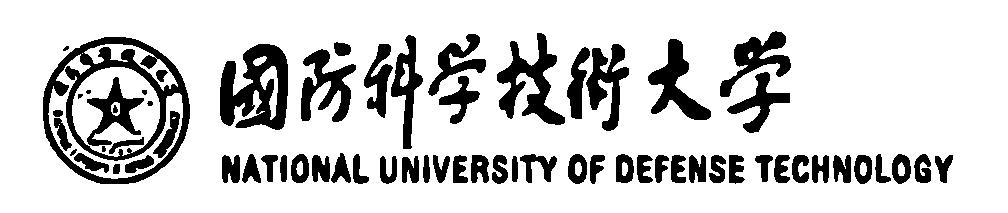
\includegraphics[height=2cm]{xhh}}
  \caption{包含子图形的大图形}
  \label{fig:big1}
\end{figure}

而下面这个例子显示并排$3\times2$的图片,见图\ref{fig:subfig:3x2}:
\begin{figure}[htb]
  \centering
  \subfloat[]{\includegraphics[width=.27\textwidth]{typography}} \qquad
  \subfloat[]{\includegraphics[width=.27\textwidth]{typography}} \qquad
  \subfloat[]{\includegraphics[width=.27\textwidth]{typography}} \qquad
  \subfloat[]{\includegraphics[width=.27\textwidth]{typography}} \qquad
  \subfloat[]{\includegraphics[width=.27\textwidth]{typography}} \qquad
  \subfloat[]{\includegraphics[width=.27\textwidth]{typography}}
  \caption{并排图片}
  \label{fig:subfig:3x2}
\end{figure}

要注意,图\ref{fig:subfig:3x2}例中
\texttt{qquad}相当于\verb|\hspace{2em}|,也就是2个字符的宽度,约0.08倍页宽,
图片宽度设定为0.27倍页宽是合适的;在该环境中,尽量不要手动换行,所以,不妨自己计算一下!

如果要把编号的两个图形并排,那么小页(minipage)就非常有用了,可以分别参考
图\ref{fig:parallel1}和图\ref{fig:parallel2}。其实这个例子和表格一节中并排
放置的表格一摸一样。
\begin{figure}[htb]
  \begin{minipage}{0.48\textwidth}
    \centering
    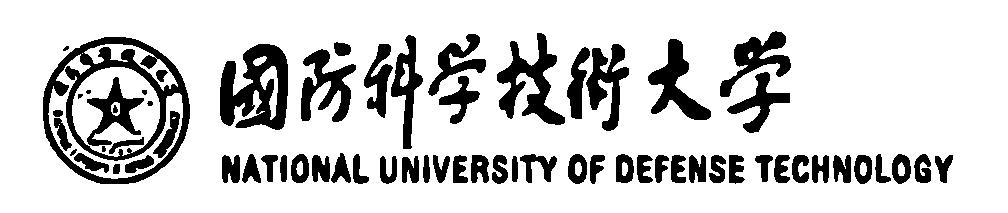
\includegraphics[height=1.2cm]{xhh}
    \caption{并排第一个图}
    \label{fig:parallel1}
  \end{minipage}\hfill
  \begin{minipage}{0.48\textwidth}
    \centering
    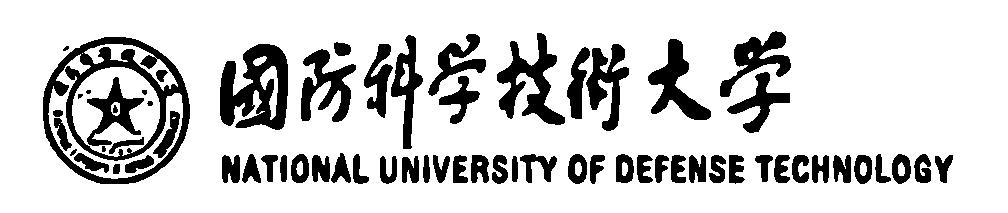
\includegraphics[height=1.2cm]{xhh}
    \caption{并排第二个图}
    \label{fig:parallel2}
  \end{minipage}
\end{figure}

图形就说这么多,因为大家在写论文是遇到的最大问题不是怎么把图插进去,
而是怎样做出专业的、诡异的、震撼的图片来,记得在这时参考前面推荐的那
些工具吧,当然必不可少的是Matlab了,至于如何加入中文标注、支持中文等等
可以上网去查,但这里{\kai 推荐一点},用好export命令,使得插入图片时尽可能的不要
缩放,保证图文的一致性。

\section{公式定理}
\label{sec:equation}
贝叶斯公式如式~(\ref{equ:chap1:bayes}),其中$p(y|\mathbf{x})$为后验;
$p(\mathbf{x})$为先验;分母$p(\mathbf{x})$ 为归一化因子,这是
实际应用中十分恐怖的一个积分式。
\begin{equation}
  \label{equ:chap1:bayes}
  p(y|\mathbf{x}) = \frac{p(\mathbf{x},y)}{p(\mathbf{x})}=
  \frac{p(\mathbf{x}|y)p(y)}{p(\mathbf{x})}
\end{equation}

论文里面公式越多,\TeX{} 就越 happy。再看一个 \textsf{amsmath} 的例子:
\newcommand{\envert}[1]{\left\lvert#1\right\rvert}
\begin{equation}\label{detK2}
  \det\mathbf{K}(t=1,t_1,\dots,t_n)=\sum_{I\in\mathbf{n}}(-1)^{\envert{I}}
  \prod_{i\in I}t_i\prod_{j\in I}(D_j+\lambda_jt_j)\det\mathbf{A}
  ^{(\lambda)}(\overline{I}|\overline{I})=0.
\end{equation}

大家在写公式的时候一定要好好看\textsf{amsmath}的文档,并参考模板中的用法:
\begin{multline*}%\tag{[b]} % 这个出现在索引中的
  \int_a^b\biggl\{\int_a^b[f(x)^2g(y)^2+f(y)^2g(x)^2]
  -2f(x)g(x)f(y)g(y)\,dx\biggr\}\,dy \\
  =\int_a^b\biggl\{g(y)^2\int_a^bf^2+f(y)^2
  \int_a^b g^2-2f(y)g(y)\int_a^b fg\biggr\}\,dy
\end{multline*}

再看\ref{equ:split}:
\begin{equation}\label{equ:split}
  \begin{split}
    C(z) &= [z^n] \biggl[\frac{e^{3/4}}{\sqrt{1-z}} +
      e^{-3/4}(1-z)^{1/2} + \frac{e^{-3/4}}{4}(1-z)^{3/2}
      + O\Bigl( (1-z)^{5/2}\Bigr)\biggr] \\
    &= \frac{e^{-3/4}}{\sqrt{\pi n}} - \frac{5e^{-3/4}}{8\sqrt{\pi
        n^3}} + \frac{e^{-3/4}}{128 \sqrt{\pi n^5}} +
    O\biggl(\frac{1}{\sqrt{\pi
        n^7}}\biggr)
  \end{split}
\end{equation}

当然了,数学中必不可少的是定理和证明:
\begin{theorem}
  \label{chapTSthm:rayleigh solution}
  假定 $X$ 的二阶矩存在:
  \begin{equation}
    O_R(\mathbf{x},F)=\sqrt{\frac{\mathbf{u}_1^T\mathbf{A}\mathbf{u}_1} {\mathbf{u}_1^T\mathbf{B}\mathbf{u}_1}}=\sqrt{\lambda_1},
  \end{equation}
  其中 $\mathbf{A}$ 等于 $(\mathbf{x}-EX)(\mathbf{x}-EX)^T$,$\mathbf{B}$ 表示协方差阵 $E(X-EX)(X-EX)^T$,$\lambda_1$
  $\mathbf{u}_1$是$\lambda_1$对应的特征向量,
\end{theorem}

对于希腊符号使用\verb|mathbf|命令可能有些问题,所以建议对符号
用\verb|bm|加粗,记得用\verb|\up<greek>|切换正体符号,下面看几个例子:
\verb|\gamma|斜体代表变量$\gamma$,\verb|\bm{\upgamma}|正体代表向量$\bm{\upgamma}$,
。\verb|\Gamma|正体代表操作符号$\Gamma$,
\verb|\bm{\Gamma}|正体粗体代表矩阵形式$\bm{\Gamma}$,
\verb|\varGamma|斜体代表变量$\varGamma$。另外对于大小写斜体的加粗可以见$\bm{\gamma}$和$\bm{\varGamma}$,
但是这两种科技论文中很少出现,这里只做测试。
非符号普通向量就用\verb|\mathbf|吧:$\mathbf{x}_k,\mathbf{X}_k$。
完整测试如下$\omega,\bm{\omega},\upomega,\bm{\upomega},\Omega,\bm{\Omega},\varOmega,\bm{\varOmega}$。

\begin{proof}
  上述优化问题显然是一个Rayleigh商问题。我们有
  \begin{align}
    O_R(\mathbf{x},F)=\sqrt{\frac{\mathbf{u}_1^T\mathbf{A}\mathbf{u}_1} {\mathbf{u}_1^T\mathbf{B}\mathbf{u}_1}}=\sqrt{\lambda_1},
  \end{align}
  其中 $\lambda_1$ 下列广义特征值问题的最大特征值:
  $$
    \mathbf{A}\mathbf{z}=\lambda\mathbf{B}\mathbf{z}, \mathbf{z}\neq 0.
  $$
  $\mathbf{u}_1$ 是 $\lambda_1$对应的特征向量。结论成立。
\end{proof}

下面来看看算法环境的定义和使用。
我们知道,故障诊断的最终目的,是将故障定位到部件,而由于信号--部件依赖矩阵的存在,因此,实质性的工作是找出由故障部件发出异常信号,
不妨称为源异常信号,而如前所述,源异常信号与异常信号依赖矩阵$\mathbf{S_a}$的全零列是存在一一对应的关系的。因此,我们只要获得了$\mathbf{S_a}$的全零列的相关信息,
也就获得了源异常信号的信息,从而能进一步找到故障源。
通过以上分析,我们构造算法\ref{alg53},用于实现非回路故障诊断。
\begin{algorithm}[htbp]
  \caption{非回路故障诊断算法}
  \label{alg53}
  \begin{algorithmic}[1]
    \REQUIRE 信号--部件依赖矩阵$\mathbf{A}$,信号依赖矩阵$\mathbf{S}$,信号状态向量$\alpha$
    \ENSURE 部件状态向量$\gamma$
    \STATE $\mathbf{P}\leftarrow\left(<\alpha>\right)$
    \STATE $\mathbf{S_{a}}\leftarrow\mathbf{P^T}\mathbf{S}\mathbf{P}$
    \FOR{$i=1$ to $S_a$的阶数$m$}
    \STATE $s_i\leftarrow s_i$的第$i$个行向量
    \ENDFOR
    \STATE $\beta_a\leftarrow\lnot \left(s_1\lor s_2\lor \cdots\lor s_m\right)^T$
    \STATE $\beta\leftarrow\mathbf{P}\beta_a$
    \STATE $\gamma\leftarrow\mathbf{A}\beta$
  \end{algorithmic}
\end{algorithm}

第一类故障回路推理与非回路故障推理是算法基本相同,稍微不同的是$\beta_a$的计算。因为第一类故障回路中的信号全部可能是源异常信号,因此我们不必计算
$\beta_a=\lnot \left(\left[s_1\lor s_2\lor \cdots\lor s_m\right]^T\right)$,而直接取$\beta_a=\underbrace{\left[\begin{array}{cccc}1&1&\cdots&1\end{array}\right]^T}_m$,将$\beta_a$代入
算法\ref{alg53},有
\[\beta=\mathbf{P}\beta_a=\mathbf{P}\underbrace{\left[\begin{array}{cccc}1&1&\cdots&1\end{array}\right]^T}_m=\alpha\]
因此一类故障回路的推理算法变得相当简单,例如算法\ref{alg54}
\begin{algorithm}[htbp]
  \caption{第一类故障回路诊断算法}
  \label{alg54}
  \begin{algorithmic}[1]
    \REQUIRE 信号--部件依赖矩阵$\mathbf{A}$,信号状态向量$\alpha$
    \ENSURE 部件状态向量$\gamma$
    \STATE $\gamma\leftarrow\mathbf{A}\alpha$
  \end{algorithmic}
\end{algorithm}

\section{参考文献}
\label{sec:bib}
当然参考文献可以直接写 bibitem,虽然费点功夫,但是好控制,各种格式可以自己随意改
写,在nudtpaper里面,建议使用JabRef编辑和管理文献,再结合\verb|bstutf8.bst|,
对中文的支持非常不错,格式也很规范。

本模板推荐使用 BIB\TeX,样式文件为 bstutf8.bst,符合学校的参考文献格式(如专利
等引用未加详细测试)。看看这个例子,关于书的\upcite{tex, companion},
还有这些\upcite{Krasnogor2004e, clzs, zjsw},关于杂志的\upcite{ELIDRISSI94,
  MELLINGER96, SHELL02},硕士论文\upcite{zhubajie, metamori2004},博士论文
\upcite{shaheshang, FistSystem01},标准文件\upcite{IEEE-1363},会议论文\upcite{DPMG,kocher99},%
技术报告\upcite{NPB2}。中文参考文献\upcite{cnarticle}\textsf{特别注意},需要在\verb|bibitem|中
增加\verb|language|域并设为\verb|zh|,英文此项可不填,之后由\verb|bstutf8|统一处理
(具体就是决定一些文献在中英文不同环境下的显示格式,如等、etc)。
若使用\verb|JabRef|,则你可按下面步骤来设置:
选择\textsf{Options}$\rightarrow$\textsf{Set Up General Fields},
在\verb|General:|后加入\verb|language|就可以了。

有时候不想要上标,那么可以这样 \cite{shaheshang},这个非常重要。

\section{代码高亮}
有些时候我们需要在论文中引入一段代码,用来衬托正文的内容,或者体现关键思路的实现。
在模板中,统一使用\texttt{listings}宏包,并且设置了基本的内容格式,并建议用户只
使用三个接口,分别控制:编程语言,行号以及边框。简洁达意即可,下面分别举例说明。

首先是设定语言,来一个C的,使用的是默认设置:
\begin{lstlisting}[language=C]
void sort(int arr[], int beg, int end)
{
  if (end > beg + 1)
  {
    int piv = arr[beg], l = beg + 1, r = end;
    while (l < r)
    {
      if (arr[l] <= piv)
        l++;
      else
        swap(&arr[l], &arr[--r]);
    }
    swap(&arr[--l], &arr[beg]);
    sort(arr, beg, l);
    sort(arr, r, end);
  }
}
\end{lstlisting}

当我们需要高亮Java代码,不需要行号,不需要边框时,可以:
\begin{lstlisting}[language=Java,numbers=none,frame=none]
// A program to display the message
// "Hello World!" on standard output

public class HelloWorld {
 
   public static void main(String[] args) {
      System.out.println("Hello World!");
   }
      
}   // end of class HelloWorld
\end{lstlisting}

细心的用户可能发现,行号被放在了正文框之外,事实上这样是比较美观的,
如果有些用户希望在正文框架之内布置所有内容,可以:
\begin{lstlisting}[language=perl,xleftmargin=2em,framexleftmargin=1.5em]
#!/usr/bin/perl
print "Hello, world!\n";
\end{lstlisting}

好了,就这么多,\texttt{listings}宏包的功能很强大也很复杂,如果需要自己定制,
可以查看其手册,耐心阅读总会找到答案。
\textbf{注意:} 当前代码环境中文注释的处理还不是很完善,对于注释请妥善处理。
在本模板中,推荐算法环境或者去掉中文的listings代码环境。
如果需要包含中文注释,不要求代码高亮,
就用\texttt{code}环境,这个环境是Verbatim的定制版,简单有效,
调用的是fancyvbr宏包,用户可在mynudt.sty中修改它的外观等等。
这里我们还可以给代码加上标签。
\begin{code}[label=hello.c]
  public class HelloWorld {
      public static void main(String[] args) {
          System.out.println("Hello World!");
        }
    }   // 世界,你好!
\end{code}

\section{符号列表}

 {\hei 前面的话:}{\kai\color{blue}
  2.2版本后默认使用nomencl环境,如果你还是希望使用传统的\verb|definition.tex|,那么只需注释掉
  顶层文件中的nomenclature即可。}

符号列表使用的是\verb|nomencl|包,自己简单定制了下,使用方法分为四步:
\begin{compactenum}
  \item 将\verb|\makenomenclature|语句放在正文前,即\verb|\begin{document}|前面;
  \item 将\verb|\printnomenclature|放在论文中,我在例子中将符号列表放在了英文摘要的
  后面,正文第一章的前面,当然,你可以根据自己的需要或者教研室的规范放置在合理的位置上,
  为了页面引用的正确,在这句话前面放上\verb|\cleardoublepage|;
  \item 使用\verb|\nomenclature|命令在论文的各个位置上添加符号定义,语法后面会讲到;
  \item 编译。编译需要首先运行一遍xelatex,之后运行
  \begin{code}
    makeindex -s nomencl.ist -o thesis.nls thesis.nlo
  \end{code}
\end{compactenum}

你可以把这句编译命令放在\verb|makepdf.bat|中第一个\verb|xelatex thesis|下面。然后
双击\verb|makepdf.bat|就可以了,论文模板中已经为你添加上了,如果你强烈不想使用
nomencl环境,只要把它注释掉(前面加\verb|rem|)就可以。
另外,由于我使用的是VIM来编辑\TeX{}代码,具体到每个编辑器(诸如WinEDT,TeXWorks等)
如何设定该命令的快捷按钮,诸位可以搜索网上的教程。

下面简单说明下\verb|\nomenclature|命令,语法为。这里插入一些随机的文字,希望
对你在阅读帮助中的思维没有什么不良的影响。
\begin{code}
  \nomenclature[<prefix>]{<symbol>}{<desc>}{<null>}
\end{code}
\verb|nomencl|模板的默认排序方法可能(大多都)不满足要求,
论文模板里,我们通过设定\verb|<prefix>|来实现符号列表的排序。
它分为两部分,比如如\verb|[Aa]|,第一个字母的含义是:
\begin{compactitem}
  \item[`A'] 符号归为拉丁字母
  \item[`G'] 希腊字母
  \item[`X'] 上标
  \item[`Z'] 下标
\end{compactitem}
每个标识后边的字幕\verb|a-z|作为当前符号组内的排列顺序,比如$\beta$就可以写成
\verb|[Gb]|,诸如此类。当然你一定注意到了,这个排序分组的设定只是为了记忆
方便,并不是强制的,因此你可以有自己的方案,比如Z是Greek,
R是Roman什么的,只要统一就好,只需记住,组间排列是按字母顺序排的。

注意符号表分四列,前三列的含义与命令中相同,
最后一列是符号定义时所在的页码。效果看例子,对于下式:
\begin{equation}\label{eq:heatflux}
  \dot{Q} = k \cdot A \cdot \Delta T
\end{equation}%
\nomenclature[Aq]{$\dot{Q}$}{heat flux}{}%
\nomenclature[Ak]{$k$}{overall heat transfer coefficient,式\eqref{eq:ohtc}}{}%
\nomenclature[Aa]{$A$}{area}{}%
\nomenclature[Al]{$L$}{length}{}%
\nomenclature[At]{$T$}{temperature}{}%
\nomenclature[At]{$\Delta T$}{temperature difference}{}%
\nomenclature[Gr]{$\gamma$}{中文测试, 以及一句很长的物理意义,很有可能超过当前栏的宽度,主要目的是看一看会不会出现某些异常情况。}{}%

或者:
\begin{equation}\label{eq:ohtc}
  \frac{1}{k} = \left[\frac{1}{\alpha _{\mathrm{i}}\,r_{\mathrm{i}}} +
  \sum^n_{j=1}\frac{1}{\lambda _j}\,
  \ln \frac{r_{\mathrm{a},j}}{r_{\mathrm{i},j}} +
  \frac{1}{\alpha _{\mathrm{a}}\,
    r_{\mathrm{a}}}\right] \cdot r_{\mathrm{reference}}
\end{equation}%
\nomenclature[Ga]{$\alpha$}{convection heat transfer coefficient}{}%
\nomenclature[Zi]{i}{in}{}%
\nomenclature[Gl]{$\lambda$}{thermal conductivity}{}%
\nomenclature[Za]{a}{out}{}%
\nomenclature[Zn]{$n$}{number of walls}{}%
\nomenclature[Zj]{$j$}{running parameter}{}%

{\hei 注意事项:}{\kai 模板中定制的nomencl格式在mynudt.sty中,默认是三栏的,分别是:
  ``符号'',``定义'',``首次出现页码'',
  注意这里的符号列表都没有单位,如果你需要额外的栏输入单位(呵呵,聪明的读者可能看出来
  了,\verb|nomenclature|命令最后一个是空的,就是用来让你赋予她各种意义的)。
  此时就需要你有一点点动手能力了(其实只要会修改表格就行),
  方法很简单,比如需要添加``国际单位制''这一栏,则
  \begin{compactenum}
    \item 论文中\verb|\nomenclature|命令的第三个参数就让他代表单位,也可留空;
    \item 将\verb|mynudt.sty|中longtable的表头添加``国际单位制''几个字,
    你也可以取其他的名字,放在那个{\kai 应该出现的}位置上;
    \item 由于增加了5个字,就把前面栏的宽度数字减5,同时设定第三栏宽度为5,
    注意这一步需要你自己调整,记得不要让表格超出边界就行。
  \end{compactenum}
}

\section{中文习惯}
\label{sec:chinese}

对于itermize过大的行间距,用户可以使用compactitem环境来替代,但是模板中不进行默认替代,
因为只有用户真正发现列表不好看才会找到这里,而且在示例文件中,
陈赓大将那个列表环境如果压缩了行距会很不好看。谢谢ZhangLei的建议!

{\hei 一个重要的提示:}
作者自己的定义命令、包等,不要放在模板里面,请放到\verb|mynudt.sty|
中,这样模板时,只要覆盖\verb|nudtpaper.cls|即可。

中文破折号为一个两个字宽垂直居中的直线,输入法直接得到的破折号是两个断开的小短线
(——),这看起来不舒服。所以模板中定义了一个破折号的命令 \verb|\pozhehao|,请看:

厚德博学,强军兴国\hfill \pozhehao{}国防科大校训


\chapter{基于hp自适应伪谱法的再入轨迹设计与分析}

飞船再入环境严苛,整个再入段受热流、过载、动压等约束的影响。应急条件下,飞船为到达目标着陆场,再入轨迹存在不同的轨迹形式。本章研究飞船再入机动可达域的快速确定问题,利用伪谱方法完成不同再入轨迹形式下的可达域确定。通过容许不同的轨迹形式,扩展再入点的范围,为应急返回提供更大的窗口。

\section{再入返回轨迹设计问题建模}
\subsection{再入动力学方程}
在探月飞船再入返回轨迹设计问题中,采用三自由度运动模型,采用“瞬时平衡假设”,认为返回器始终以配平攻角飞行,且侧滑角为零。考虑地球自转,圆球假设下,忽略地球扁率和侧滑角等的影响,在半速度系下建立运动方程,以时间为自变量的飞船无动力再入动力学方程满足
\begin{equation}
	\left\{
	\begin{aligned}
		\frac{\dif r}{\dif t}=       & v \sin \theta                                                           \\
		\frac{\dif \lambda}{\dif t}= & \frac{v \cos \theta \sin \psi}
		{r \cos \phi}                                                                                          \\
		\frac{\dif \phi}{\dif t}=    & \frac{v \cos \theta \cos \psi}{r}                                       \\
		\frac{\dif v}{\dif t}=       & -D-g \sin \theta +\omega_e^2r\cos\phi \sin\theta \cos\phi-
		\omega_e^2r\cos\phi\cos\theta\sin\phi\cos\sigma                                                        \\
		\frac{\dif\theta}{\dif t} =  & \frac{L\cos\sigma}{v}+(\frac{v}{r}-
		\frac{g}{v})\cos\theta+2\omega_e\cos\phi\sin\sigma                                                     \\
		                             & {}+\frac{\omega_e^2r\cos\phi\cos\theta\cos\phi}{v}                      \\
		\frac{\dif\psi}{\dif t} =    & \frac{L\sin\sigma}{v\cos\theta}+\frac{v\sin \psi\cos \theta\tan\phi}{r}
		-2\omega_e(\cos\phi\tan\theta\cos\sigma-\sin\phi)                                                      \\
		                             & {}+\frac{\omega_e^2r}{\cos\theta}sin\phi\cos\phi\sin\sigma
	\end{aligned}
	\right.
\end{equation}
其中,$r$为地心距,$\lambda$和$\phi$为经纬度,$v$为相对地球速度,$\theta$为当地速度倾角,表征速度与当地水平的夹角,以及$\psi$为速度方位角,表征速度在当地水平面内的投影与当地正北方向的夹角,顺时针为正;$\sigma$为控制量倾侧角,反映了升力对铅锤面的倾斜;$ \omega_e $为地球自转角速度,$L$,$D$为再入过程中的升力阻力加速度,满足
\begin{align}
	L & =\frac{C_L\rho v^2S}{2m} \\
	D & =\frac{C_D\rho v^2S}{2m}
\end{align}
其中:$ C_L $和$ C_D $为气动升力系数和气动阻力系数,$ \rho $为大气密度,$ m $为飞行器质量,$ S $为飞船的参考面积。

大气密度$ \rho $可采用指数模型、多阶段拟合公式和美国US1976标准大气模型等,考虑到精度和计算速度的要求,最终采用多阶段的拟合公式,更多可参考\upcite{贾沛然-1993-远程火箭弹道学}。
\begin{equation}
	\rho=\rho_0 e^{-\beta h}
\end{equation}

\subsection{约束分析}
因探月返回器高速再入的特点,过载和热流等约束十分苛刻。为了保证再入过程的安全,根据约束的性质划分为两类:过程约束和终端约束。
\subsubsection{过程约束}
\begin{enumerate}
	\item 热流约束\par
	      高超声速气动加热对热防护系统(TPS)的影响,为避免飞行器被烧毁,因此需对飞行器再入过程中的热流密度进行限制。
	      通常采用驻点热流密度作为约束指标,计算公式如下:
	      \begin{equation}
		      \dot{Q} = k_s\left(\frac{\rho}{\rho_{0}}\right)^{0.5}\left(\frac{v}{V_{c}}\right)^{m}
	      \end{equation}
	      其中,$ k_s $为热流相关常数,$ V_c=7.9\mathrm{km/s} $为参考的第一宇宙速度,$ m $可取3或3.15,本文中取3.15
	\item 过载约束\par
	      考虑到内部结构、材料的限制,需要对过载进行限制,要求瞬时过载小于最大允许过载,即
	      \begin{equation}
		      n=\sqrt{{{L}^{2}}+{{D}^{2}}}\le {{n}_{\max }}
	      \end{equation}
	      其中,$ n_{\max} $为最大允许过载值。
	\item 动压约束\par
	      动压对控制系统的影响和侧向稳定性的要求,
	      \begin{equation}
		      q=\frac{1}{2} \rho V^{2} \leq q_{\max }
	      \end{equation}
	\item 跃起高度约束\par
	      此外,为防止跳出高度过高导致任务失败,路径约束还应包括一个高度约束。这里设定最大高度不超过300km,
	      \begin{equation}
		      h<h_{\max}
	      \end{equation}
	\item 控制量约束\par
	      控制量倾侧角受限于执行机构,飞船的控制能力有限,实际倾侧角机动不可能瞬时完成,需要对倾侧角和倾侧角变化速率进行限幅,即
	      \begin{equation}
		      \left\{
		      \begin{aligned}
			      \abs{\sigma}       & \leq \sigma_{\max}       \\
			      \abs{\dot{\sigma}} & \leq \dot{\sigma}_{\max} \\
		      \end{aligned} \right.
	      \end{equation}
\end{enumerate}

\subsubsection{终端约束}
对于再入问题中的终端约束,包含起始点和终点的状态约束。起始点处的状态在分析中通常为给定值,在初始时刻$ t_0 $状态满足
\begin{equation}
	\left\{ \begin{aligned}
		h(t_0)=h_0,\lambda(t_0)=\lambda_0,\phi(t_0)=\phi_0 \\
		v(t_0)=v_0,\theta(t_0)=\theta_0,\psi(t_0)=\psi_0
	\end{aligned} \right.
\end{equation}

终点处根据研究问题可分为固定终点和自由终点两种情况,数学上表达为:
\begin{enumerate}
	\item 固定终点的约束条件\par
	      终点处位置固定,但速度和速度倾角存在范围约束,即:
	      \begin{equation}
		      \left\{ \begin{aligned}
			      h(t_f) & =h_{f}, \lambda(t_f)=\lambda_{f}, \phi(t_f)=\phi_{f}       \\
			      v      & \geq v_{f}, \theta_{\min } \leq \theta \leq \theta_{\max }
		      \end{aligned}\right.
	      \end{equation}
	\item 自由终点的约束条件\par
	      对于求解可达域等问题时,终点不固定,通常约束设置为:
	      \begin{equation}
		      h(t_f)=h_{f}, v \geq v_{f}, \theta_{\min } \leq \theta \leq \theta_{\max }
	      \end{equation}
\end{enumerate}

\section{hp自适应伪谱法的求解策略}
hp自适应伪谱法是伪谱方法的一种,求解再入问题在计算速度有较大优势。hp自适应伪谱法主要包含两部分内容:伪谱化离散和hp自适应网格细化。
\subsection{LGR离散化方法}
%在绪论中介绍轨迹优化问题描述
首先将在连续时间$ [t_0,t_f] $上的问题划分为$ K $个子区间,记第$ k $个子区间为$ [t_{k-1},t_k] $,有$ t_0<t_1<t_2<\ldots<t_k $。对于
第k个子区间,首先需要将时域$ t\in[t_{k-1},t_k] $,转换到$ \tau \in [-1,1] $,即:
\begin{equation}
	\tau = \frac{2 t-\left(t_{k-1}+t_{k}\right)}{t_{k}-t_{k-1}}
	\label{eq:time Trans}
\end{equation}

经过区间划分后,$ [t_0,t_f] $时间内的连续优化问题可以表述为:
\begin{enumerate}
	\item 动力学方程
	      \begin{equation}
		      \frac{\dif \boldsymbol{x}^{(k)}(\tau)}{\dif \tau}=\frac{t_{k}-t_{k-1}}{2} f\left(\boldsymbol{x}^{(k)}(\tau), \boldsymbol{u}^{(k)}(\tau)\right), \quad(k=1, \cdots, K)
	      \end{equation}
	\item 目标函数
	      \begin{equation}
		      J=\Phi\left(\boldsymbol{x}^{(1)}(-1), t_{0}, \boldsymbol{x}^{(K)}(+1), t_{K}\right)+\sum_{k=1}^{K} \frac{t_{k}-t_{k-1}}{2} \int_{t_{0}}^{t_{f}} g\left(\boldsymbol{x}^{(k)}(\tau), \boldsymbol{u}^{(k)}(\tau)\right) d \tau
	      \end{equation}
	\item 路径约束
	      \begin{equation}
		      \frac{t_{k}-t_{k-1}}{2} \boldsymbol{C}\left(\boldsymbol{x}^{(k)}(\tau), \boldsymbol{u}^{(k)}(\tau)\right) \leq 0 \quad(k=1, \cdots, K)
	      \end{equation}
	\item 边界条件
	      \begin{equation}
		      \phi\left(\boldsymbol{x}^{(1)}(-1), t_{0}, \boldsymbol{x}^{(K)}(+1), t_{K}\right)=0
	      \end{equation}
\end{enumerate}

引入区间划分后,附加产生额外的内点约束:
\begin{equation}
	\phi\left(\boldsymbol{x}^{(1)}(-1), t_{0}, \boldsymbol{x}^{(K)}(+1), t_{K}\right)=0
\end{equation}

进一步,需要对问题进行离散化求解。Radau伪谱法的配点为Legendre-Gauss-Radau(LGR)点,LGR点相对于原点是不对称的,并且不是唯一的,
可以使用初始点或终点来定义它们。一般的LGR点配置在 $ [t_{k-1},t_k) $上(包含起点),将其归一化后,即端点$ \tau_{N_k+1}^{(k)}=+1 $为非配点。区间内的离散点为$ -1=\tau_1<\tau_2<\cdots<\tau_{N_k}<\tau_{N_k+1} $,此处省略上标$ k $。
对于任意一个子区间$  [t_{k-1},t_k] $,取$ N_k $个LGR点,取插值点为$ N_k $个LGR点与终端点$ \tau_{N_k+1}^{(k)}=+1 $,状态量的近似可以表示为:
\begin{equation}
	\boldsymbol{x}^{(k)}(\tau) \approx \boldsymbol{X}^{(k)}(\tau)=\sum_{j=1}^{N_{k}+1} \boldsymbol{X}_{j}^{(k)} L_{j}^{(k)}(\tau)
	\label{eq:state}
\end{equation}
其中,简记$ \boldsymbol{X}_{j}^{(k)}=\boldsymbol{X}^{(k)}\left(\tau_{j}^{(k)}\right)$,$ \quad L_{j}^{(k)}(\tau) $为Lagrange插值
基函数:
\begin{equation}
	L_{j}^{(k)}(\tau)=\prod_{i=1, i \neq j}^{N_{k}+1} \frac{\tau-\tau_{i}^{(k)}}{\tau_{j}^{(k)}-\tau_{i}^{(k)}}
\end{equation}

获得状态量的近似后,进一步对于动力学方程的状态导数可以近似为:
\begin{equation}
	\frac{\dif \boldsymbol{x}^{(k)}(\tau)}{\dif \tau} \approx \frac{\dif \boldsymbol{X}^{(k)}(\tau)}{\dif \tau}=\sum_{j=1}^{N_{k}+1} \boldsymbol{X}_{j}^{(k)} \dot{L}_{j}^{(k)}(\tau)
\end{equation}

状态量的近似通过在$ N_k+1 $个插值点处的Lagrange插值多项式近似,对于控制量通过在$ N_k $个配点处插值获得,有:
\begin{equation}
	\boldsymbol{u}^{(k)}(\tau) \approx \boldsymbol{U}^{(k)}(\tau)=\sum_{i=1}^{N_{k}} \boldsymbol{U}_{i}^{(k)}\widetilde{L}_{i}^{(k)}(\tau)
	\label{eq:control}
\end{equation}
其中$ \widetilde{L}_{i}^{(k)}(\tau) $与$ L_{j}^{(k)}(\tau) $具有类似的形式,此处不再列出。

经过\eqref{eq:state}-\eqref{eq:control}的处理,连续时间上的原最优控制问题可转化为其离散形式:
\begin{enumerate}
	\item 动力学方程\par
	      在配点处,原动力学微分方程约束转换为代数约束形式,表达为:
	      \begin{equation}
		      \sum_{j=1}^{N_{k}+1} \boldsymbol{X}_{j}^{(k)} D_{i j}^{(k)}-\frac{t_{k}-t_{k-1}}{2} \boldsymbol{f}_{i}^{(k)}=0, \quad\left(i=1, \cdots, N_{k}, k=1, \cdots, K\right)
	      \end{equation}
	      其中,$\boldsymbol{f}_{i}^{(k)}=\boldsymbol{f}\left(\boldsymbol{X}_{i}^{(k)}, \boldsymbol{U}_{i}^{(k)}\right)$,简记$ \boldsymbol{U}_{i}^{(k)}=\boldsymbol{U}^{(k)}\left(\tau_{i}^{(k)}\right)$,式中:
	      \begin{equation}
		      D_{i j}^{(k)}=\dot{L}_{j}^{(k)}\left(\tau_{i}^{(k)}\right) \quad\left(i=1, \cdots, N_{k}, j=1, \cdots, N_{k}+1\right)
	      \end{equation}
	      $ \left\{D_{i j}^{(k)}\right\} $为区间$ k $内大小$ N_k\times (N_k+1) $的微分矩阵,通常可以利用差分近似。
	\item 目标函数\par
	      目标函数转化为
	      \begin{equation}
		      J=\Phi\left(\boldsymbol{X}^{(1)}(-1), t_{0}, \boldsymbol{X}_{N_{K}+1}^{(K)}, t_{K}\right)+\sum_{k=1}^{K} \sum_{j=1}^{N_{K}} \frac{t_{k}-t_{k-1}}{2} w_{j}^{(k)} g_{j}^{(k)}
	      \end{equation}
	      其中,$w_{j}^{(k)}=\int_{-1}^{1} L_{j}^{(k)}(\tau) d \tau$为第k个子区间上的Legendre-Gauss权重,$g_{j}^{(k)}=g\left(\boldsymbol{X}_{j}^{(k)}, \boldsymbol{U}_{j}^{(k)}\right)$。
	\item 路径约束\par
	      \begin{equation}
		      \frac{t_{k}-t_{k-1}}{2} \boldsymbol{C}^{(k)}\left(\boldsymbol{X}_{i}^{(k)}, \boldsymbol{U}_{i}^{(k)}\right) \leq 0 \quad\left(i=1, \cdots, N_{k}, k=1, \cdots, K\right)
	      \end{equation}
	\item 边界条件\par
	      \begin{equation}\phi\left(\boldsymbol{X}^{(1)}(-1), t_{0}, \boldsymbol{X}_{N_{K}+1}^{(K)}, t_{K}\right)=0\end{equation}
	      同时离散化引入的附加内点约束变为:
	      \begin{equation}
		      \boldsymbol{X}_{N_{k}+1}^{(k)}=\boldsymbol{X}_{1}^{(k+1)}, \quad(k=1, \ldots, K-1)
	      \end{equation}
\end{enumerate}

文献【19】从近似精度和计算效率等方面对上述三种伪谱法进行了比较。 Radau伪谱法和Gauss伪谱法在状态变量、控制变量和共轭变量的近似精度上均优于 Legendre伪谱法,同时, Gauss伪谱法对共轭变量边界值的估计精度高于Radau伪谱法,且在处理含初始和终端约束的问题上具有优势。在计算效率方面,求解相同规模问题时三种方法耗时差别不大。

\subsection{hp自适应网格细化方法}
最早hp方法发展于求解偏微分方程中的有限元方法,进一步被引入到求解最优控制问题,解决不连续点上收敛速度慢的问题。hp方法是为提高求解精度和收敛速度的一种p方法和h方法的混合算法。p方法是保持通过提高插值多项式的阶次进行求解,全局的伪谱方法就是典型的p方法;h方法通过划分区间,固定区间内插值多项式的阶次,通过细化区间求解问题。hp方法能够综合p方法在光滑解条件下的指数收敛速度优势并且只在不连续的区域或者解发生突变处细化区间。研究\upcite{Darby-2011-Directtrajectoryoptimization,Darby-2011-hpadaptivepseudospectral}也表明hp方法相比于p方法和h方法,能够有效降低近似的维度。

hp方法的基本思想是:从初始网格出发,对每段的近似误差进行估计,通过增大插值多项式的阶次和对当前区间进行划分的方法对当前网格进行细化,重复直至精度满足要求。

\subsubsection{误差评估}
为衡量在区间$ [t_{k-1},t_k] $内动力学方程约束的满足情况,首先定义区间内的一系列评估误差的检验点,取为相邻配点的中点,有:
\begin{equation}
	\bar{t}_{i}=\frac{t_{i}+t_{i+1}}{2} \quad\left(i=1, \ldots, N_{k}-1\right)
\end{equation}

在这些检验点上,通过\eqref{eq:state}和\eqref{eq:control}获得这些点处的状态量$ \overline{\boldsymbol{X}} $和控制量$ \overline{\boldsymbol{U}} $的估计值,分别为$ (N_k-1)\times n $和$ (N_k-1)\times m $的矩阵,这里$ n $和$ m $分别为状态量和控制量的个数。
\begin{equation}
	\overline{\boldsymbol{X}}=\left[\begin{array}{c}
			\boldsymbol{X}\left(\bar{t}_{1}\right) \\
			\vdots                                 \\
			\boldsymbol{X}\left(\bar{t}_{N_{k}-1}\right)
		\end{array}\right], \quad \overline{\boldsymbol{U}}=\left[\begin{array}{c}
			\boldsymbol{u}\left(\bar{t}_{1}\right) \\
			\vdots                                 \\
			\boldsymbol{u}\left(\bar{t}_{N_{k}-1}\right)
		\end{array}\right]
\end{equation}

进一步,通过式\eqref{eq:time Trans}对时间进行时域变换,得到$ \tau=\left(\bar{\tau}_{1}, \ldots, \bar{\tau}_{N_{k}-1}\right) \in[-1,1] $。计算动力学约束的误差$ \boldsymbol{R} $为
\begin{equation}
	\boldsymbol{R}=\left|\bar{\boldsymbol{ D }} \bar{\boldsymbol{X}}-\frac{t_{k}-t_{k-1}}{2} \boldsymbol{F}\left(\overline{\boldsymbol{X}}, \overline{\boldsymbol{U}}, \tau ; \boldsymbol{p}, t_{k-1}, t_{k}\right)\right| \in \mathbb{R}^{\left(N_{k}-1\right) \times n}
	\label{eq:residual func}
\end{equation}
$ \boldsymbol{R} $为$ (N_k-1)\times n  $的矩阵,矩阵中的每列元素都代表了对应状态在配点间的违反程度。

% where denotes the absolute value of each element of the matrix R. The elements of the matrix R will be referred to as the midpoint residuals of the dynamics at the midpoints of the collocation points and the matrix R itself will be referred to as the midpoint residual matrix. Each column of the matrix r provides a measure of the amount by which the state violates the collocation equations at the midpoints between two collocation points in segment s

记矩阵$ \boldsymbol{R} $中最大元素所在列为$ \boldsymbol{r} $,$ \boldsymbol{r} $可以表示为
\begin{equation}
	\boldsymbol{r}=\left[\begin{array}{c}
			r\left(\bar{t}_{1}\right) \\
			\vdots                    \\
			r\left(\bar{t}_{N_{k}-1}\right)
		\end{array}\right]
\end{equation}

由于$ \boldsymbol{r} $中包含最大偏差处的信息,可以作为进一步划分区间或者增加插值多项式阶次的依据。

进一步,记$ \bar{r}$为向量,$ \boldsymbol{r} $的算术平均值,即:
\begin{equation}
	\bar{r}=\frac{\sum_{i=1}^{N_{k}-1} r\left(\bar{t}_{i}\right)}{N_{k}-1}
\end{equation}
定义
\begin{equation}
	\boldsymbol{\beta}=\left[\begin{array}{c}
			\beta\left(\bar{t}_{1}\right) \\
			\vdots                        \\
			\beta\left(\bar{t}_{N_{s}-1}\right)
		\end{array}\right]=\left[\begin{array}{c}
			r\left(\bar{t}_{1}\right) / \bar{r} \\
			\vdots                              \\
			r\left(\bar{t}_{N_{s}-1}\right) / \bar{r}
		\end{array}\right]
\end{equation}
$ \bm{\beta} $为尺度变换后的在检验点处的偏差向量,代替$ \boldsymbol{r} $作为后续细化策略的依据。
\subsubsection{细化策略}
对于向量$ \bm{\beta} $,存在两种情况,分别对应细化区间和增加插值多项式阶次两种策略:
\begin{enumerate}
	\item 当$ \bm{\beta} $中的元素都很小时,认为在区间$ k $中没有误差特别大的点,为提高式\eqref{eq:residual func}精度,增加插值多项式阶次;
	\item 当$ \bm{\beta} $中的元素存在一些点处的误差明显大于其他元素时,则认为在区间$ k $中存在误差特别大的点,在该处对区间进一步细化。
\end{enumerate}

下面讨论在上述策略下如何增加阶次和网格划分的具体策略。定义$ \varepsilon $为设定的误差阈值,当式\eqref{eq:residual func}的最大值大于$ \varepsilon $,认为需要对该区间进行划分或者增加插值多项式阶次。设定一个阈值$ \eta$衡量向量$ \bm{\beta} $中的元素大小,可以认为:
\begin{enumerate}
	\item 增加插值阶次\par
	      当向量$ \bm{\beta} $中的所有元素都小于设定的阈值$ \eta $时,动力学约束的误差认为来自插值多项式,因此增加插值多项式阶次,表示为:
	      \begin{equation}
		      N^{(n+1)}_k=N^{(n)}_k+L
	      \end{equation}
	      其中,$ N^{(n)}_k $表示第$ n $次迭代中,区间$ k $的配点个数,$ L $为设定的增加配点个数。
	\item 细化区间\par
	      当向量$ \bm{\beta} $中的存在一些点处的值大于设定的阈值$ \eta $时,将超出阈值的点设为新的分段点,另外对于存在图\ref{fig:hp-sketch}这一类邻近点均超过阈值的情况,仅将其中最大值对应的点设为新的分段点。
\end{enumerate}
\begin{figure}[htb]
	\begin{small}
		\begin{center}
			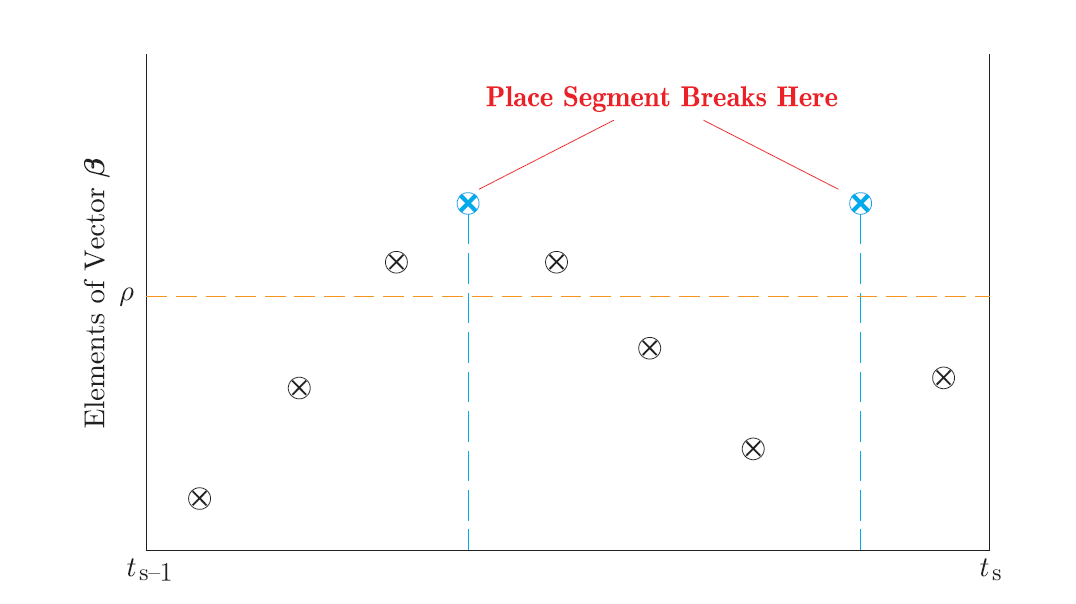
\includegraphics[width=0.8\textwidth]{figures/hp-sketch}
		\end{center}
		\caption{hp网格细化示意图}
		\label{fig:hp-sketch}
	\end{small}
\end{figure}
更多可技术细节参考\upcite{Patterson-2014-GPOPSIIMATLAB}。

\section{伪谱法快速可达域计算与分析}

可达域的计算目的是得到飞船在固定初始状态下,获得其机动包络能力。
\subsection{可达域求解策略}
求解再入可达域问题可以表示为求解不同纵程条件下的最大横程问题。即包含两步:
\begin{compactenum}
	\item 求解纵程优化问题,获得纵程的范围;
	\item 在给定纵程下,求解横程优化问题。
\end{compactenum}

首先定义纵程与横程的


\subsection{纵向航程范围获取}
最大最小纵程的轨迹设计

\subsection{可达域方法的计算结果}
程序测试通过,做出类似这样的图的效果
\begin{figure}[htb]
	\begin{minipage}{0.48\textwidth}
		\centering
		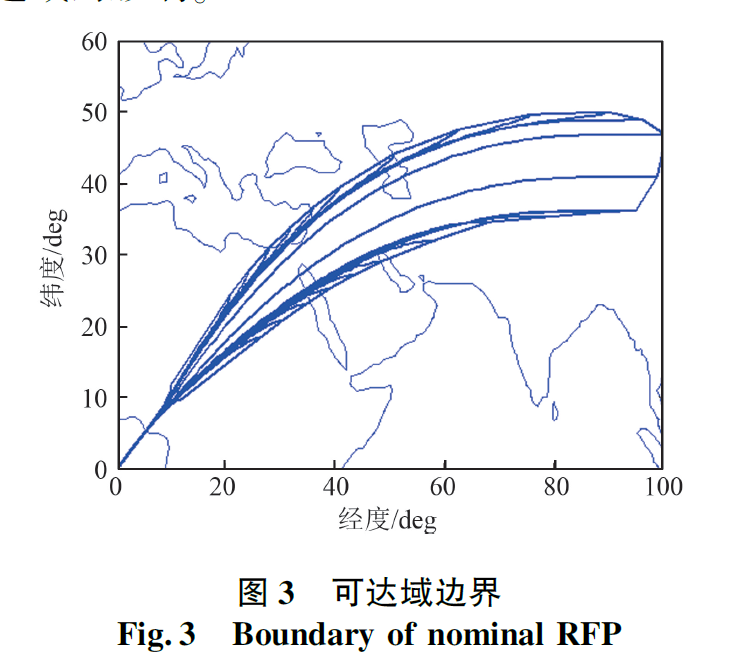
\includegraphics[width=\textwidth]{footboundary.png}
		\caption{并排第一个图}
		\label{fig:parallel1}
	\end{minipage}\hfill
	\begin{minipage}{0.48\textwidth}
		\centering
		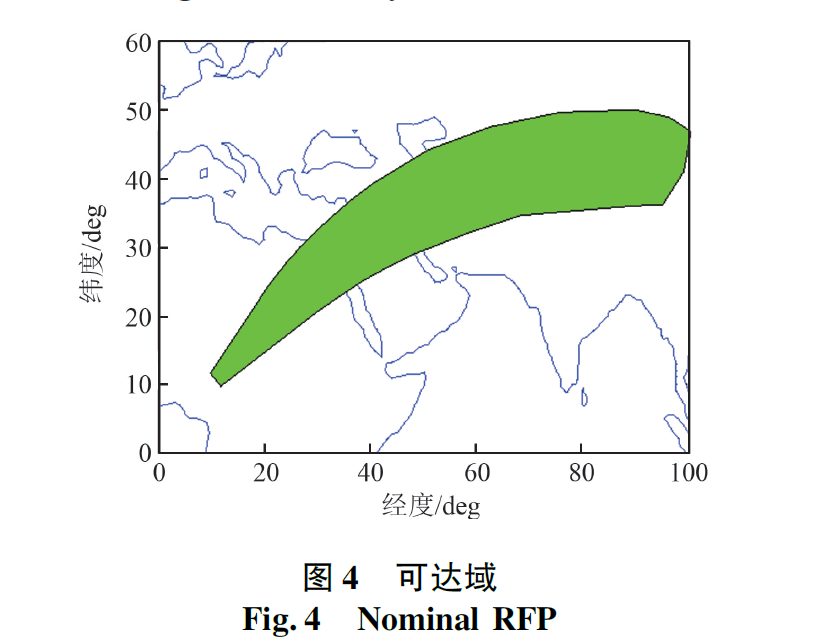
\includegraphics[width=\textwidth]{footboundary2.png}
		\caption{并排第二个图}
		\label{fig:parallel2}
	\end{minipage}
\end{figure}

\begin{figure}[htb]
	\begin{minipage}{0.48\textwidth}
		\centering
		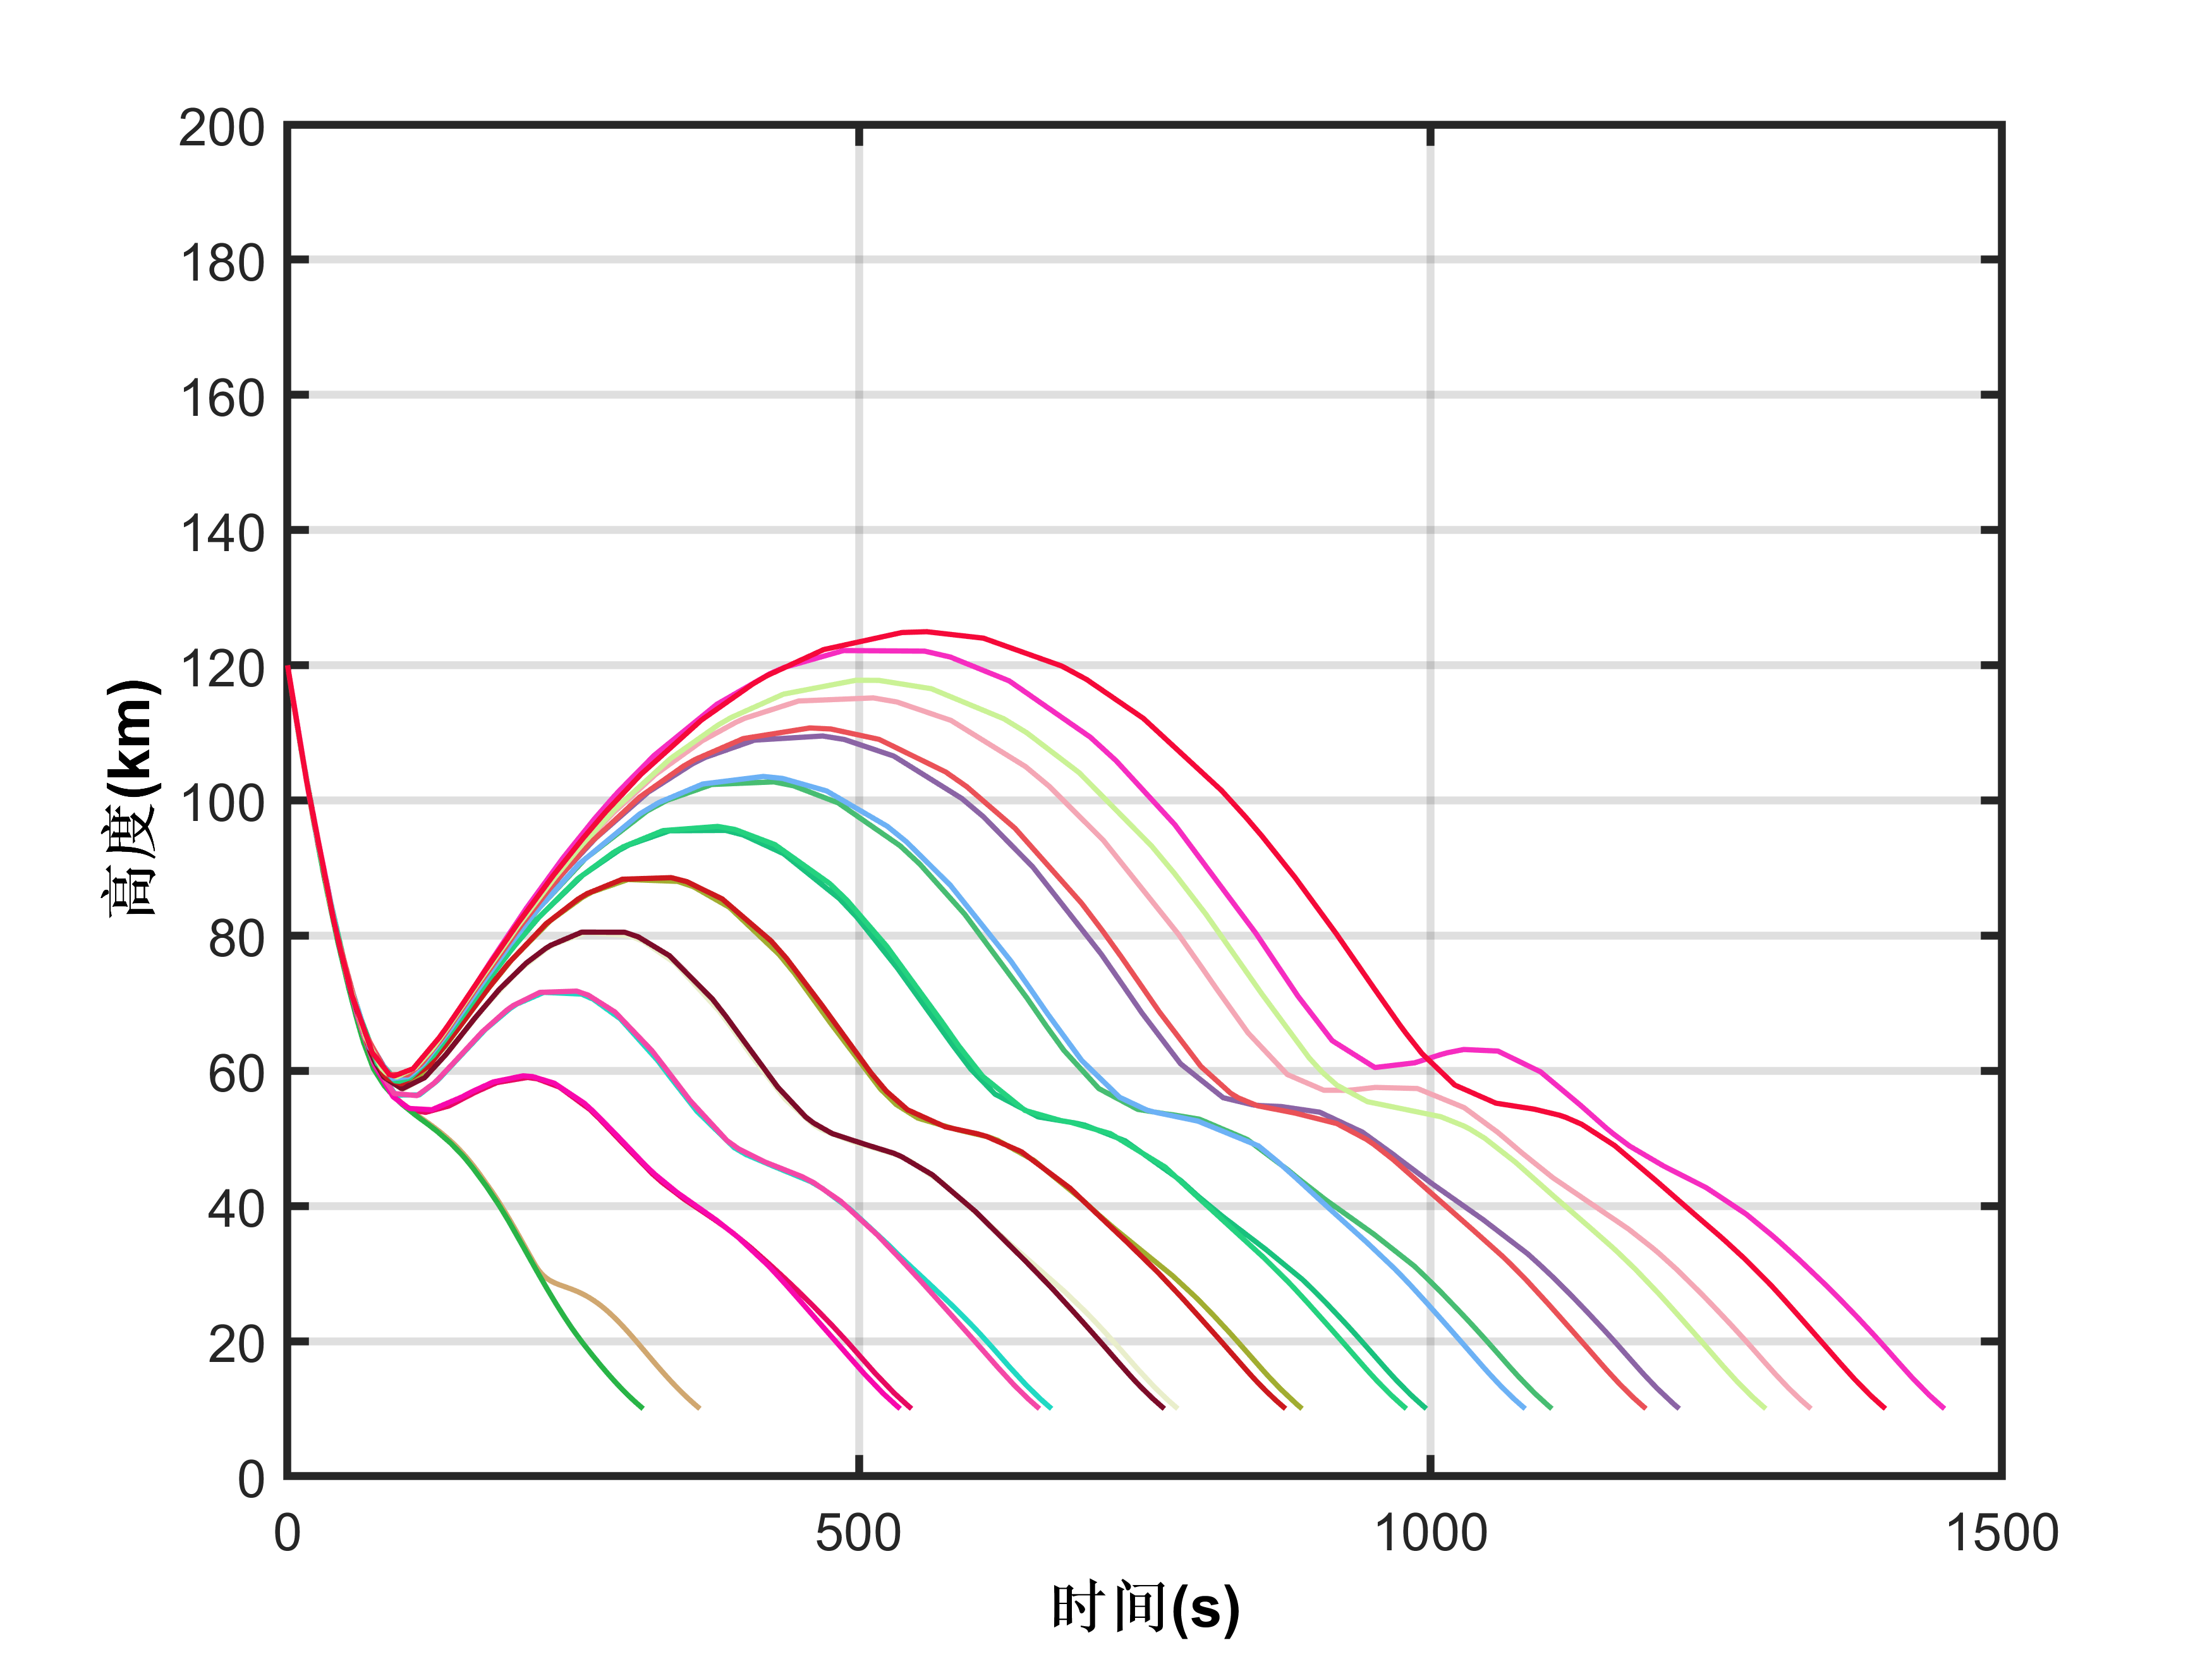
\includegraphics[width=\textwidth]{1.png}
		\caption{并排第一个图}
		\label{fig:parallel1}
	\end{minipage}\hfill
	\begin{minipage}{0.48\textwidth}
		\centering
		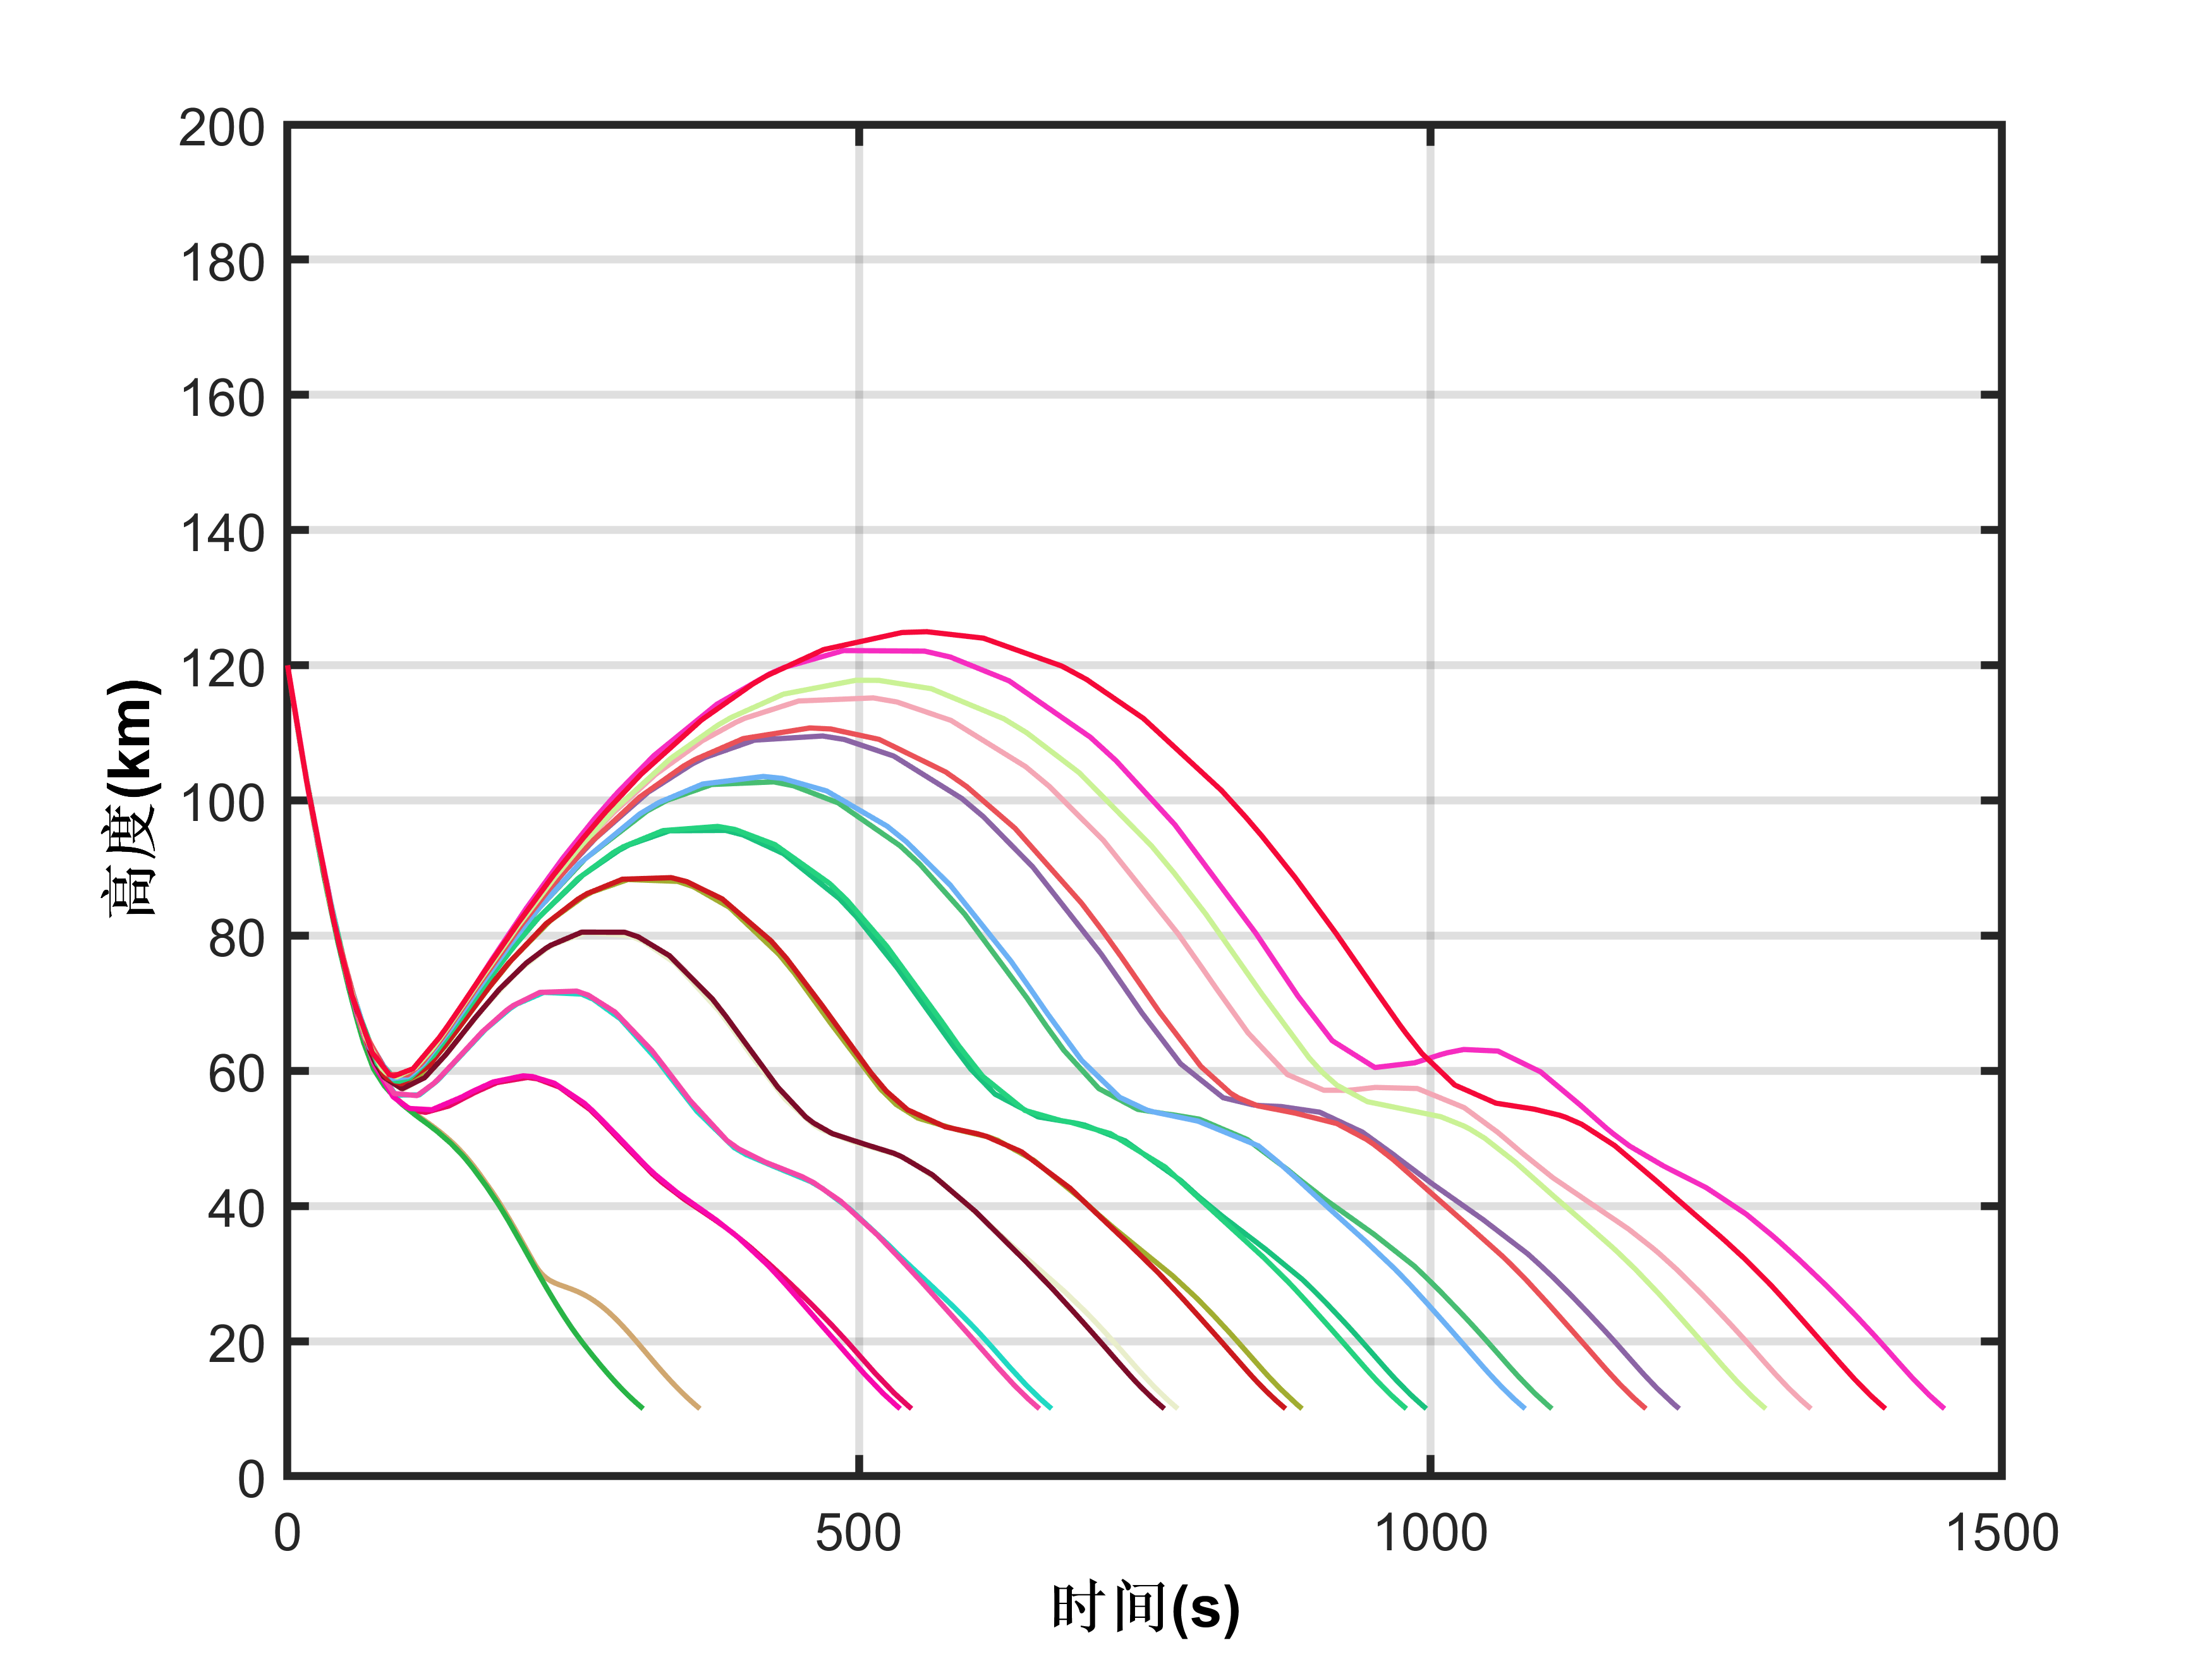
\includegraphics[width=\textwidth]{1.png}
		\caption{并排第二个图}
		\label{fig:parallel2}
	\end{minipage}
\end{figure}

\section{短航程再入轨迹设计结果对比}
\subsection{短航程再入解析轨迹设计}
短航程设计简要介绍??
\subsection{结果对比分析}
分析其中最短航程对应的参数情况,对应返回最为恶劣的情况

% \chapter{月地返回轨道设计}
\section{月地转移轨道设计}
\subsection{双二体假设下中止轨道计算模型}

设$t_A$时刻进行中止机动,中止点$A$在月心惯性坐标系下的坐标为$r_A^L=[x_A^L\quad y_A^L\quad z_A^L]$,给定出口点经度$\lambda_C$和纬度$\phi_C$,则出口点在月心惯性坐标系下的坐标为

对于跳跃式再入的航天器,初始再入点是冉人轨道的初始点,其位置、速度、速度角将决定再入飞行特性。初始再入点又是月地转移轨道的目标点,受到月地转移轨道的约束。影响初始再入点参数的主要因素有返回时刻、再入角的大小和再入轨道倾角的要求、升轨或降轨到达地球。


\subsection{瞄准参数分析}
\subsubsection{再入角}
再入角只有在飞船到达大气边界才有意义,再入角满足如下的计算方程
\begin{equation}
	\tan \gamma_\mathrm{e}=\frac{1}{R_\mathrm{P}\sqrt{1+e}}\sqrt{-{R_\mathrm{P}}^2(1+e)+2R_\mathrm{e}R_\mathrm{P}-{R_e}^2(1-e)}
\end{equation}
其中,$R_\mathrm{P}$为近地点地心距,$R_\mathrm{e}$为再入点EI的地心距,$e$为地心转移轨道的倾角。
如果$e=1$,则近似有
\begin{equation}
	R_{\mathrm P}=R_{\mathrm{e}}\cos^2\gamma_{\mathrm{e}}
\end{equation}
\subsubsection{再入点经纬度}
再入点处的纬度由月球的赤纬、方向角和再入角决定,与月球的返回时刻相关。再入点的经度受地球自转影响,为短周期项,是返回时间的函数。因此,通过搜索返回时刻与返回时间能够分别满足要求。
\subsubsection{方向角}
方位角和倾角都可以描述再入飞行方向,但是倾角不能确定唯一的飞行方向,因此这里选择方位角描述。不考虑再入过程的横向机动,给定着陆点$F$经纬度$(\theta_{\mathrm f},\phi_{\mathrm f})$和再入点经纬度$(\theta_{\mathrm e},\phi_{\mathrm e})$,根据球面三角公式可以求出瞄准着陆点的标称再入速度方位角,作为月球转移轨道的瞄准参数。

由于防热的原因,设计者希望以较小的大气相对速度再入,而逆行轨道的大气相对速度比顺行轨道更大,所以要求方位角范围在$0\degree\sim 180\degree$之间。

\section{双二体模型下的返回轨道初步设计方法}
在月地转移过程中,飞行器受到地球和月球的引力场作用,地球、月球与飞行器构成限制性三体问题,一般情况下无解析解。

双二体模型是对限制性三体模型的近似,可以分别计算地心段和月心段轨道的解析解,然后将两段轨道拼接为一个整体,也即圆锥曲线拼接法。该方法是
种无需轨道积分的纯代数计算方法,具有收敛速度快的优点,适用于需要大规模计算的参数特性分析,或者作为高精度计算的初值估计。

本节针对月球返回问题建立适应于此问题的新的数学模型。在新的数学模型中,选择物理意乂明确的轨道参数代替出口点经纬度来作为设计变量,可以避免设计参数物理意义不明确的缺点。

\subsection{用到的坐标系}

\begin{enumerate}[label=\arabic*)]
	\item 地心白道系$O_E-XYZ$

		  原点为地心$ O_E $,$ xy $平面为某瞬时$ t_0 $时刻(航天器到达出口点时刻)的白道面, $ x $轴为该时刻由月心指向地心的方向,$ z $轴垂直$ t_0 $时刻的白道面,方向与该时刻月球绕地球公转动量矩方向一致
	\item 月心白道系$O_M-XYZ$

			坐标原点平移,方向与地心白道系$O_E-XYZ$一致。
	\item 月心J2000坐标系

			原点在月心$ O_M $,三轴指向与地心惯性系一致。在此坐标系中与月心白道系转换方便,故用于定义初始月球轨道(LLO轨道根数)
	\item 地心惯性系(ECI)
	\item 地固系(ECF)
\end{enumerate}
\subsection{优化参数(设计变量)选择}
传统的地月空间圆锥曲线拼接方法均采用影响球出口点(或入口点)经度纬度$ \lambda_B,\phi_B $作为设计变量,采用这两个参数可以实现地心段和月心段轨道的拼接计算但作为设计变量却存在不足:1)物理意义不如轨道根数明确,获得它们的分布特性需要通过大量仿真计算;2)需要利用这两个参数结合其它设计变量去推导出地心段和月心段两部分轨道参数,这些轨道参数中有很多本来可以作为输入条件给出的。通过出口点经纬度导出后,在设计模型中有些输入参数却只能作为等式约束存在,增加了额外的等式约束。

{\color{red}参考,}将初始的LLO轨道参数作为模型的输入参数,选择设计变量为:
\begin{enumerate}[label=\arabic*)]
	\item 航天器到达出口点时刻$t_B$
	\item 月心白道系下的出口点纬度幅角$u$
	\item 月心白道系下出口点速度大小$v_{si}$
	\item 加速点A处的速度倾角$\Theta_A$
	      % 在不考虑异面变轨,认为加速脉冲方向沿LO速度方向施加,速度倾角$\Theta_A=0\degree$
\end{enumerate}

\subsection{返回轨道设计动力学模型}
考虑将月球停泊轨道倾角和升交点赤经作为输入条件,同时采用新的具有明显物理意义的设计变量,建立新的返回轨道数学模型

在地心位置矢量$\bm{r}$可表示为
\begin{equation}
	\bm{r}=\bm{r}_M+\bm{r}_{si}
\end{equation}
其中,$\bm{r}_{si}$为B点的月心位置矢量,$\bm{r}_M$为月球的地心位置矢量

出口点速度矢量$v$在地心白道系中矢量表达式为
\begin{equation}
	\bm{v}=\bm{v}_\mathrm{m}+\bm{v}_\mathrm{si}
\end{equation}
其中$ \bm{v}_\mathrm{si} $为出口点速度在月心白道系中矢量,$ \bm{v}_\mathrm{m} $为是月球速度在地心白道系中矢量。

\begin{figure}[htb]
	\centering
	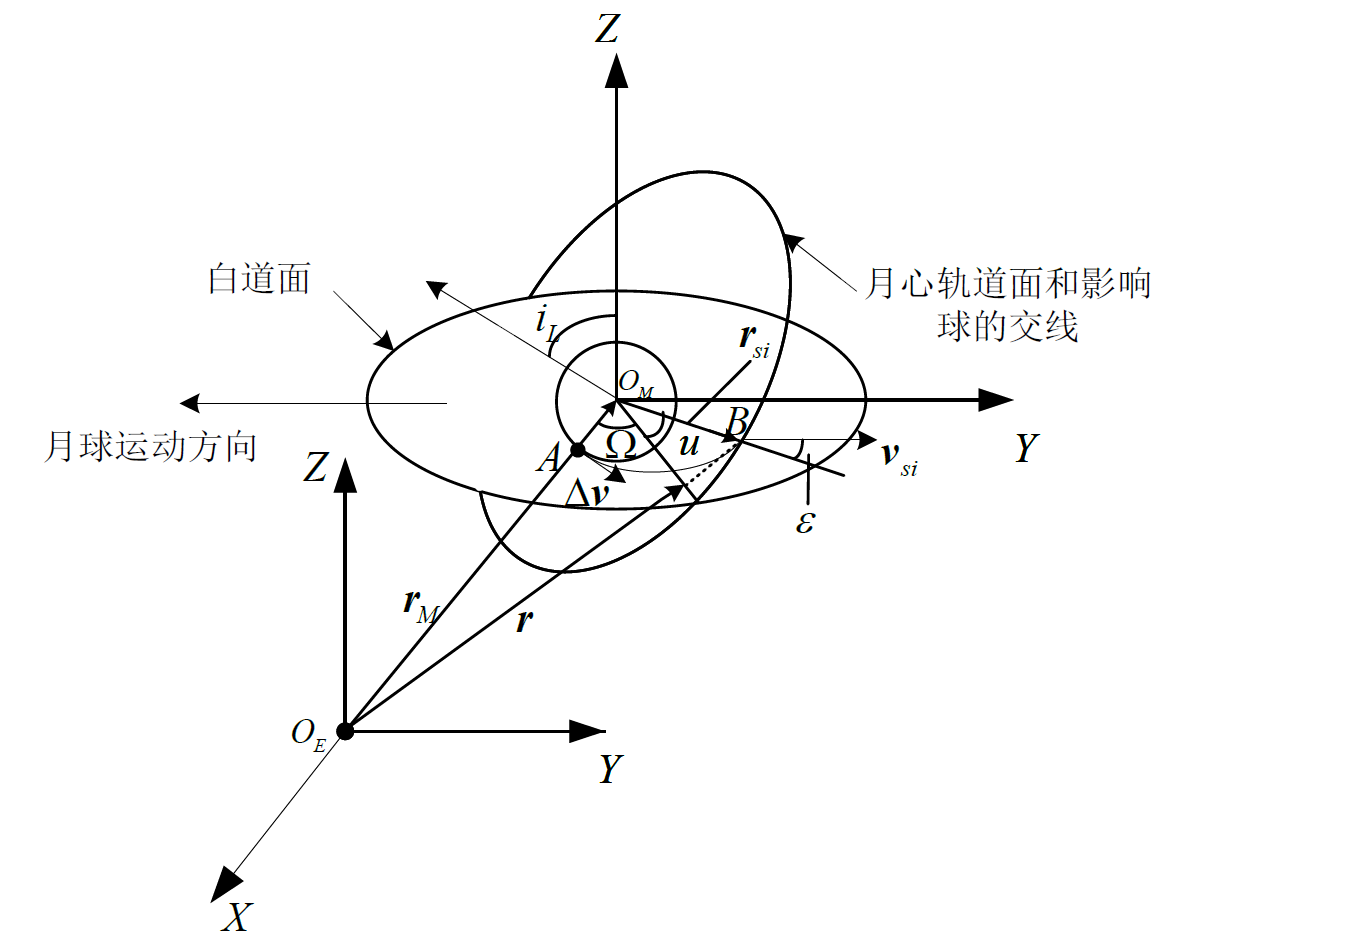
\includegraphics[scale=0.4]{double_two_body_para.png}
	\caption{双二体轨道参数示意图}
	\label{fig:double_two_body_para}
\end{figure}

月心白道系下的出口点位置矢量$\bm{r}_{si}$可以表示为
\begin{equation}
	\bm{r}_{si}^{\mathrm{EMP}}=R_3(-\Omega)R_1(-i)R_3(-u)\left[\begin{array}{c}
			r_{si} \\0\\0
		\end{array}\right]
\end{equation}



进一步考虑月球轨道的非圆性问题,即采用高精度地月运动关系下的圆锥曲线拼接模型进行求解,而不是认为月球是绕地球作匀速圆周运动,这样做在一定程度上能够提髙计算精度。在利用圆锥曲线拼接法求解过程中,所涉及到任何时刻的月球位置和速度均以 JPL DE405星历表为基础得到。$ \bm{v}_\mathrm{m} $可表示为
\begin{equation}
	\bm{v}_\mathrm{m}^{\mathrm{EMP}}=M_{\mathrm{ECI}}^{\mathrm{EMP}}\bm{v}_\mathrm{m}^{\mathrm{ECI}}
\end{equation}
其中,$ M_{\mathrm{ECI}}^{\mathrm{EMP}} $为当前时刻地心惯性系到地心白道系的旋转矩阵。
% 此处的表述选择优化,增加上标EMP,无标记仅代表矢量

假设脉冲$ \Delta v $在LLO面内时,即不考虑异面变轨,$ \bm{v}_\mathrm{si}  $也在月心轨道面内,可以表达为
\begin{equation}
	\begin{aligned}
		\boldsymbol{v}_{\mathrm{si}}^{\mathrm{EMP}}= & R_{3}(-\Omega) R_{1}(-i) R_{3}(-u)  \left[\begin{array}{c}
				v_{s i} \cos \varepsilon \\
				0                        \\
				0
			\end{array}\right]                      \\
		{}                            & +R_{3}(-\Omega) R_{1}(-i) R_{3}\left(-u-90^{\circ}\right)\left[\begin{array}{c}
				v_{s i} \sin \varepsilon \\
				0                        \\
				0
			\end{array}\right]
	\end{aligned}
\end{equation}
其中,$ \epsilon $为出口点位置矢量和速度矢量夹角,可通过月心轨道能量守恒和角动量守恒得到
\begin{equation}\sin \varepsilon=\frac{r_{A}}{r_{s i}} \sqrt{1+\frac{2 \mu_{M}}{r_{A} v_{s i}^{2}}\left(1-\frac{r_{A}}{r_{s i}}\right)} \cos \Theta_{A}\end{equation}

通过将地心位置矢量和速度矢量在地心惯性系下表达,进一步可以求解其他地心轨道参数,近地距、再入角、再入点经纬度、方位角等。初值问题,Lagrange法等,相关计算公式参考郗,相关函数有基础,整理。

\subsection{约束条件分析}
\begin{enumerate}
	\item 优化变量的范围
	
	$ v_1 \leq v_{si} \geq v_{\max} \to f(\Delta v_{\max})$
	\item 航程约束分析

		经过上述计算,可以得到再入点处的位置和速度矢量(地心J2000),着陆点$ (\lambda_f,\phi_f) $已知,通过地固系转换到地心J2000。其中,需要估计再入段航程所用时间。
		根据位置矢量计算航程角$ \delta_R $,
\end{enumerate}
\section{月地返回轨道精确设计结果}
借助STK实现

% 
%%% Local Variables:
%%% mode: latex
%%% TeX-master: "../main"
%%% End:

\begin{ack}
  衷心感谢导师 xxx 教授和 xxx 副教授对本人的精心指导。他们的言传身教将使我终生受益。

  感谢 \nudtpaper{},它的存在让我的论文写作轻松自在了许多,让我的论文格式规整漂亮了许多。

\end{ack}


\cleardoublepage
\phantomsection
\addcontentsline{toc}{chapter}{参考文献}
\bibliographystyle{bstutf8}
\bibliography{ref/refs,ref/own_ref}

% \begin{resume}
\ifreview
该论文作者在学期间取得的阶段性成果(学术论文等)已满足我校博士学位评阅相关要求。为避免阶段性成果信息对专家评价学位论文本身造成干扰,特将论文作者的阶段性成果信息隐去。
\else
  \section*{发表的学术论文} % 发表的和录用的合在一起

  \begin{enumerate}[label={[\arabic*]}]
  \addtolength{\itemsep}{-.36\baselineskip}%缩小条目之间的间距,下面类似
  \item Yang Y, Ren T L, Zhang L T, et al. Miniature microphone with silicon-
    based ferroelectric thin films. Integrated Ferroelectrics, 2003,
    52:229-235. (SCI 收录, 检索号:758FZ.)
  \item 杨轶, 张宁欣, 任天令, 等. 硅基铁电微声学器件中薄膜残余应力的研究. 中国机
    械工程, 2005, 16(14):1289-1291. (EI 收录, 检索号:0534931 2907.)
  \item 杨轶, 张宁欣, 任天令, 等. 集成铁电器件中的关键工艺研究. 仪器仪表学报,
    2003, 24(S4):192-193. (EI 源刊.)
  \item Yang Y, Ren T L, Zhu Y P, et al. PMUTs for handwriting recognition. In
    press. (已被 Integrated Ferroelectrics 录用. SCI 源刊.)
  \item Wu X M, Yang Y, Cai J, et al. Measurements of ferroelectric MEMS
    microphones. Integrated Ferroelectrics, 2005, 69:417-429. (SCI 收录, 检索号
    :896KM.)
  \item 贾泽, 杨轶, 陈兢, 等. 用于压电和电容微麦克风的体硅腐蚀相关研究. 压电与声
    光, 2006, 28(1):117-119. (EI 收录, 检索号:06129773469.)
  \item 伍晓明, 杨轶, 张宁欣, 等. 基于MEMS技术的集成铁电硅微麦克风. 中国集成电路, 
    2003, 53:59-61.
  \end{enumerate}

  \section*{研究成果} % 有就写,没有就删除
  \begin{enumerate}[label=\textbf{[\arabic*]}]
  \addtolength{\itemsep}{-.36\baselineskip}%
  \item 任天令, 杨轶, 朱一平, 等. 硅基铁电微声学传感器畴极化区域控制和电极连接的
    方法: 中国, CN1602118A. (中国专利公开号.)
  \item Ren T L, Yang Y, Zhu Y P, et al. Piezoelectric micro acoustic sensor
    based on ferroelectric materials: USA, No.11/215, 102. (美国发明专利申请号.)
  \end{enumerate}
\fi
\end{resume}

% 最后,需要的话还要生成附录,全文随之结束。
\appendix
\backmatter
% % TeX
\chapter{模板提供的希腊字母命令列表}

大写希腊字母:
\begin{table}[htbp]
\centering
\begin{tabular}{llll}
\toprule
$\Gamma$~\verb|\Gamma| & $\Lambda$~\verb|\Lambda| & $\Sigma$~\verb|\Sigma| & $\Psi$~\verb|\Psi| \\
$\Delta$~\verb|\Delta| & $\Xi$~\verb|\Xi| & $\Upsilon$~\verb|\Upsilon| & $\Omega$~\verb|\Omega| \\
$\Theta$~\verb|\Theta| & $\Pi$~\verb|\Pi| & $\Phi$~\verb|\Phi| & \\
\midrule
$\varGamma$~\verb|\varGamma| & $\varLambda$~\verb|\varLambda| & $\varSigma$~\verb|\varSigma| & $\varPsi$~\verb|\varPsi| \\
$\varDelta$~\verb|\varDelta| & $\varXi$~\verb|\varXi| & $\varUpsilon$~\verb|\varUpsilon| & $\varOmega$~\verb|\varOmega| \\
$\varTheta$~\verb|\varTheta| & $\varPi$~\verb|\varPi| & $\varPhi$~\verb|\varPhi| & \\
\bottomrule
\end{tabular}
\end{table}

小写希腊字母:
\begin{table}[htbp]
\centering
\begin{tabular}{llll}
\toprule
$\alpha$~\verb|\alpha| & $\theta$~\verb|\theta| & $o$~\verb|o| & $\tau$~\verb|\tau| \\ 
$\beta$~\verb|\beta| & $\vartheta$~\verb|\vartheta| & $\pi$~\verb|\pi| & $\upsilon$~\verb|\upsilon| \\ 
$\gamma$~\verb|\gamma| & $\iota$~\verb|\iota| & $\varpi$~\verb|\varpi| & $\phi$~\verb|\phi| \\ 
$\delta$~\verb|\delta| & $\kappa$~\verb|\kappa| & $\rho$~\verb|\rho| & $\varphi$~\verb|\varphi| \\ 
$\epsilon$~\verb|\epsilon| & $\lambda$~\verb|\lambda| & $\varrho$~\verb|\varrho| & $\chi$~\verb|\chi| \\ 
$\varepsilon$~\verb|\varepsilon| & $\mu$~\verb|\mu| & $\sigma$~\verb|\sigma| & $\psi$~\verb|\psi| \\ 
$\zeta$~\verb|\zeta| & $\nu$~\verb|\nu| & $\varsigma$~\verb|\varsigma| & $\omega$~\verb|\omega| \\ 
$\eta$~\verb|\eta| & $\xi$~\verb|\xi| & $\varkappa$~\verb|\varkappa| & $\digamma$~\verb|\digamma| \\ 
\midrule
$\upalpha$~\verb|\upalpha| & $\uptheta$~\verb|\uptheta| & $\mathrm{o}$~\verb|\mathrm{o}| & $\uptau$~\verb|\uptau| \\ 
$\upbeta$~\verb|\upbeta| & $\upvartheta$~\verb|\upvartheta| & $\uppi$~\verb|\uppi| & $\upupsilon$~\verb|\upupsilon| \\ 
$\upgamma$~\verb|\upgamma| & $\upiota$~\verb|\upiota| & $\upvarpi$~\verb|\upvarpi| & $\upphi$~\verb|\upphi| \\ 
$\updelta$~\verb|\updelta| & $\upkappa$~\verb|\upkappa| & $\uprho$~\verb|\uprho| & $\upvarphi$~\verb|\upvarphi| \\ 
$\upepsilon$~\verb|\upepsilon| & $\uplambda$~\verb|\uplambda| & $\upvarrho$~\verb|\upvarrho| & $\upchi$~\verb|\upchi| \\ 
$\upvarepsilon$~\verb|\upvarepsilon| & $\upmu$~\verb|\upmu| & $\upsigma$~\verb|\upsigma| & $\uppsi$~\verb|\uppsi| \\ 
$\upzeta$~\verb|\upzeta| & $\upnu$~\verb|\upnu| & $\upvarsigma$~\verb|\upvarsigma| & $\upomega$~\verb|\upomega| \\ 
$\upeta$~\verb|\upeta| & $\upxi$~\verb|\upxi| & & \\ 
\bottomrule
\end{tabular}
\end{table}

希腊字母属于数学符号类别,请用\verb|\bm|命令加粗,其余向量、矩阵可用\verb|\mathbf|。


\end{document}
